%%%%%%%%%%%%%%%%%%%%%%%%%%%%%%%%%%%%%%%%%%%%%%%%%%%%%%%%%%%%%%%%%%%%%%%%%%%%%%%%
% M.Tech. (Data Science) Thesis Project -- Phase I Evaluation Report
% Batch 2025--27, Semester III
%
% The MTP runs over two semesters. Phase I = the work done in Semester III
% (July--November 2026), evaluated through this report and a poster.
% Phase II = the work done in Semester IV, evaluated through the thesis and an
% oral presentation.
%
% HOW TO USE THIS TEMPLATE
%  1. Upload this file, references.bib and neurips_2026.sty (from
%     https://neurips.cc) to a new Overleaf project. Compile with pdfLaTeX
%     + BibTeX.
%  2. Do NOT change the style file, margins, font size or line spacing.
%  3. Blue "Guidance" boxes explain what each section must contain. Read them,
%     write your text, then switch them off with \showguidefalse (below)
%     before you submit. The page limit applies with the boxes switched off.
%  4. Page limit: the Conclusion section (Section 9) must end within the first
%     10 pages. References, the declarations and the appendix may follow and
%     do not count towards the limit.
%  5. Submit a single PDF named  <RollNo>_MTP1_Report.pdf
%%%%%%%%%%%%%%%%%%%%%%%%%%%%%%%%%%%%%%%%%%%%%%%%%%%%%%%%%%%%%%%%%%%%%%%%%%%%%%%%

\documentclass{article}
\usepackage[hidelinks]{hyperref}
\usepackage{graphicx}
\usepackage{booktabs}

% Always use the "preprint" option: it shows your name and removes line numbers.
% Do not use the default (anonymous) or "final" options.
\usepackage[preprint]{neurips_2026}

\usepackage[utf8]{inputenc} % allow utf-8 input
\usepackage[T1]{fontenc}    % use 8-bit T1 fonts
\usepackage{hyperref}       % hyperlinks
\usepackage{url}            % simple URL typesetting
\usepackage{booktabs}       % professional-quality tables
\usepackage{amsmath}        % equations
\usepackage{amssymb}        % blackboard math symbols
\usepackage{nicefrac}       % compact symbols for 1/2, etc.
\usepackage{microtype}      % microtypography
\usepackage{xcolor}         % colors
\usepackage{graphicx}       % figures

% Footer on the first page (replaces the NeurIPS "Preprint" notice).
\makeatletter
\def\@noticestring{M.Tech.\ (Data Science) Thesis Project, Phase~I Evaluation
  Report (work done in Semester~III), IIT Guwahati, 2026.}
\makeatother

% ---------------------------------------------------------------------------
% Guidance boxes. Set to \showguidefalse before submission.
\newif\ifshowguide
% \showguidetrue
\showguidefalse
\newcommand{\guide}[1]{%
  \ifshowguide
    \par\medskip\noindent
    \fcolorbox{blue!50}{blue!4}{%
      \begin{minipage}{\dimexpr\linewidth-2\fboxsep-2\fboxrule\relax}
        \small\color{blue!55!black}\textbf{Guidance.} #1
      \end{minipage}}%
    \par\medskip
  \fi}
% ---------------------------------------------------------------------------

\title{On the Complementarity of C-band \& S-band SAR Images}

% Student on the first line; supervisors side by side on the second line.
% If you have a third supervisor, uncomment the third block.
\author{%
  R. Virinchi \\
  Roll No.: 254161009 \\
  M.Tech.\ in Data Science (Batch 2025--27) \\
  Indian Institute of Technology Guwahati \\
  \texttt{r.virinchi@iitg.ac.in}
  \AND
  Supervisor 1: Dr. Manish Bhatt \\
  Electrical and Electronics Engineering \\
  IIT Guwahati \\
  \texttt{manishb@iitg.ac.in}
  \And
  Supervisor 2: Dr. Neeraj Kumar Sharma \\
  MFSDSAI \\
  IIT Guwahati \\
  \texttt{neerajs@iitg.ac.in}
  % \And
  % Supervisor 3: Prof.\ Name \\
  % Department / School \\
  % IIT Guwahati \\
  % \texttt{supervisor3@iitg.ac.in}
}

\renewcommand{\topfraction}{0.9}
\renewcommand{\bottomfraction}{0.8}
\renewcommand{\textfraction}{0.07}
\renewcommand{\floatpagefraction}{0.85}

\begin{document}

\maketitle

\begin{abstract}
  \guide{One paragraph, at most 200 words. Answer, in this order: (i) What problem
  are you solving and why does it matter? (ii) What is your approach? (iii) What
  have you achieved so far in Phase~I (give at least one concrete number if you
  have results)? (iv) What will you do in Semester~IV? Do not cite references
  here.}
  High-resolution monitoring of seasonal snow cover in the Himalayas is vital for hydrological runoff forecasting, hydropower scheduling, agricultural irrigation, and disaster management. While optical satellites accurately map snow under clear skies, persistent mountain cloud cover obscures 50\% to 70\% of winter accumulation and spring melt observations, hence, cloud-penetrating Synthetic Aperture Radar (SAR) techniques need to be developed. This work presents a weakly supervised deep learning framework that transfers 20m snow labels generated from Sentinel-2 optical imagery to Sentinel-1 SAR imagery. In Phase~I, 18-scene Himalayan dataset spanning $58{,}740\text{ km}^2$ was curated and three different model training experiments were done each with a different combination of input channels. The 6-channel model gave snow F1-score of 69.27\% (96.48\% Overall F1) on same basin different date (temporal transfer) and 50.42\% (89.83\% Overall F1) on different basin different date (spatial+temporal transfer). In Semester~IV, integration of S-band SAR will be done in order to test whether S-band has enough new information to complement C-band and subsequently a novel approach to combine both of them will be proposed.
\end{abstract}

\noindent\textbf{Keywords:} Snow cover segmentation, C-band, S-band, SAR.

%===============================================================================
\section{Introduction}
\label{sec:intro}

\guide{About one page. A reader who stops after this section should know exactly
what you are doing and how far you have got. Use the four paragraphs below and
keep their headings. Throughout this report, \emph{Phase~I} means the MTP work
done in Semester~III, and \emph{Phase~II} the work to be done in Semester~IV.}

\paragraph{Motivation.}
Accurate estimation of seasonal snow cover extent is critical for regional climate modeling, water resource management, hydroelectric power generation, and disaster forecasting.
% lemke2007observations, viviroli2007mountains, rouhier2018regionalisation, deng2024development, immerzeel2019importance, 
Globally, seasonal snow covers up to 49\% of the Northern Hemisphere land surface during midwinter, stores 75\% of terrestrial freshwater, and reflects 80\% to 90\% of incoming solar radiation due to its high albedo (0.80--0.90) \citep{briand2026weakly}. In the Hindu Kush--Himalayan (HKH) and Tibetan Plateau regions, seasonal snow and glacier melt feed 10 major Asian river systems that directly sustain nearly 2 billion people with water for drinking, irrigation, and hydropower \citep{li2020gap}. However, optical satellites such as MODIS and Sentinel-2 are obstructed by cloud cover for over 50\% to 70\% of the winter accumulation and spring melt seasons in high-mountain regions, for instance, \citet{briand2026weakly} documented 52\% missing daily optical observations across a single water year in the French Alps, with cloud obscuration peaking during snowfall events. Synthetic Aperture Radar (SAR) penetrates clouds regardless of solar illumination hence C-band SAR images have been extensively used in the past to predict snow cover under cloud cover. However, C-band alone is not sufficient because it is highly sensitive to sparse vegetation in 3000-5000m elevation range. Until now no other alternatives were present but with the launch of NISAR satellite, for the first time S-band SAR is publicly accessible. S-band is not affected as much by sparse vegetation due to longer wavelength however it isn't sufficient alone either because it is less sensitive to shallow/fine-grained dry snow than C-band and will underestimate the amount of snow present above 5000m altitude. Hence, it is essential to find a way to combine C and S band SAR images and take advantage of their complementarity to train a model that can estimate snow cover better than models trained on either band alone. This has never been attempted in the past because S-band SAR was not available at large scale but with the recent launch of NISAR satellite, S-band has become available over entire Himalayan region hence enabling this study.
% \citep{nagler2016advancements}

\paragraph{Problem statement.}
Given co-registered multi-temporal dual-polarization SAR backscatter imagery ($\sigma^0_{\text{VV}}, \sigma^0_{\text{VH}}$), snow-free summer reference backscatter ($\sigma^0_{\text{VV,ref}}, \sigma^0_{\text{VH,ref}}$), and static topographic features (elevation and slope), the problem is to train a weakly supervised convolutional neural network using optical snow labels derived from Sentinel-2 via LIS algorithm (Figure~\ref{fig:concept}) so that the model accurately segments binary snow cover and then determine whether combining S-band and C-band SAR improves segmentation over existing models that are trained only on single SAR band.

\begin{figure}[!htbp]
  \centering
  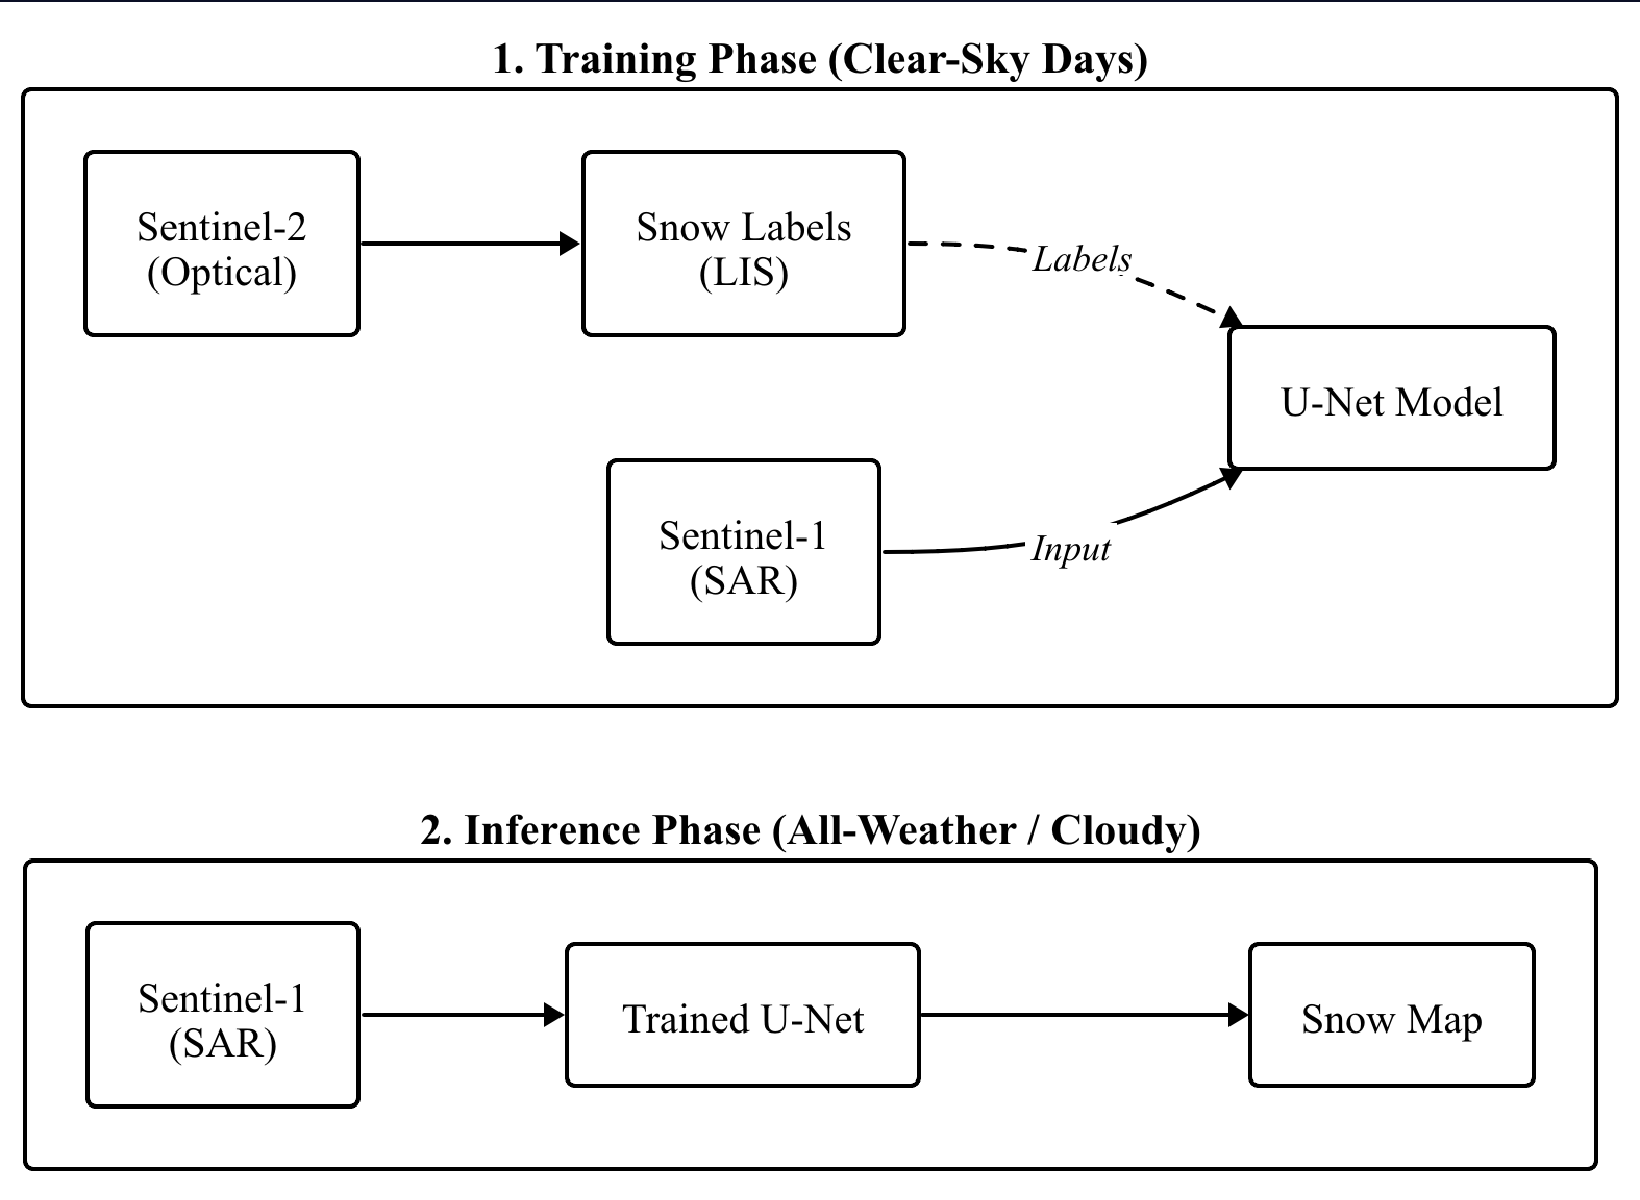
\includegraphics[width=0.66\textwidth]{figures/weak_supervision_concept.pdf}
  \vspace{-4pt}
  \caption{Weakly supervised training and all-weather SAR inference concept.}
  \label{fig:concept}
\end{figure}

\paragraph{Objectives.}
The objectives of the full project and their current status are summarized in Table~\ref{tab:objectives}.

\begin{table}[h]
  \caption{Thesis objectives and their status at the end of Phase~I.}
  \label{tab:objectives}
  \centering
  \begin{tabular}{p{0.06\linewidth}p{0.66\linewidth}p{0.20\linewidth}}
    \toprule
    No. & Objective & Status \\
    \midrule
    O1 & Generate 20\,m weak supervision snow labels in the Himalayas from Sentinel-2 optical imagery and DEM data using the Let-It-Snow (LIS) algorithm while masking cloud-obscured pixels. & Completed \\
    O2 & Establish a C-band Sentinel-1 SAR snow segmentation baseline (U-Net) and evaluate the addition of Rayleigh MLE snow-free summer references ($\sigma^0_{\text{VV,ref}}, \sigma^0_{\text{VH,ref}}$) and topographic features (Elevation, Slope). & Completed \\
    O3 & Develop an S-band SAR snow segmentation pipeline and compare standalone S-band against C-band performance across elevation zones. & Planned (Sem.~IV) \\
    O4 & Fuse C-band and S-band SAR data to evaluate whether S-band is complementary to C-band and whether combining both frequencies improves snow segmentation accuracy. & Planned (Sem.~IV) \\
    O5 & Package everything into a GUI app for demonstration. Write and submit final report. & Planned (Sem.~IV) \\
    \bottomrule
  \end{tabular}
\end{table}

\paragraph{Work done in Phase~I (Semester~III).}
During Semester~III, data preprocessing, pipeline engineering and C-band model experiments were performed. (Objectives O1 and O2):
\begin{itemize}
  \item Surveyed the literature on optical and SAR snow mapping, benchmarking the methodology against the state-of-the-art weakly supervised framework of \citet{briand2026weakly}.
  \item Curated and co-registered an 18-scene Himalayan multi-sensor dataset (Sentinel-1 IW GRDH SAR, Sentinel-2 L2A optical, and Copernicus 30\,m DEM) at 10\,m UTM resolution across a primary training/validation basin ($\sim 58{,}740\text{ km}^2$) and an unseen spatial transfer test region ($\sim 22{,}200\text{ km}^2$).
  \item Automated optical weak-label generation using the Let-It-Snow (LIS) algorithm \citep{simon2018algorithm} and SAR radiometric/terrain correction via ESA SNAP (SeNtiel Application Platform).
  \item Implemented a Rayleigh Maximum Likelihood Estimator (MLE) with a permanent-snow safeguard across summer scenes to construct snow-free reference images ($\sigma^0_{\text{VV,ref}}, \sigma^0_{\text{VH,ref}}$).
  \item Trained and evaluated three progressive C-band U-Net models (2-channel raw SAR, 4-channel SAR + MLE, and 6-channel SAR + MLE + DEM), improving validation $\text{F1}_{\text{Snow}}$ from 56.84\% to 69.27\% and unseen test $\text{F1}_{\text{Snow}}$ from 43.34\% to 50.42\% while achieving 100\% accuracy in snow-free valleys ($<3000\text{ m}$).
\end{itemize}

%===============================================================================
\section{Literature Review}
\label{sec:lit}

\guide{About 1--1.5 pages. Organise the review by \emph{theme or approach}, not
paper by paper; use \texttt{\textbackslash paragraph\{\}} headings for themes.
For each theme, say what the methods do, what they achieve and where they fall
short. Prefer recent peer-reviewed work and key original papers; cite with
\texttt{\textbackslash citet} / \texttt{\textbackslash citep}. End with a short
paragraph titled \emph{Research gap} that states, in your own words, what is
missing and how your project addresses it. A comparison table of closely related
works is encouraged.}

% \citep{dozier1984snow, dozier1989spectral}

\paragraph{Snow cover estimation using optical images.}
Optical snow mapping exploits the strong contrast between snow's high visible reflectance and low Short-Wave Infrared (SWIR) reflectance (Figure~\ref{fig:s2_lis_demo}). \citet{hall1995development} formalized the Normalized Difference Snow Index, applying a fixed threshold of 0.40 in the operational 500\,m MODIS product. However, \citet{harer2018need} demonstrated that a fixed 0.40 NDSI threshold causes local classification errors of up to 24.1\% at 20--30\,m resolution in rugged alpine terrain. To address this, \citet{simon2018algorithm} developed the Let-It-Snow (LIS) algorithm for the 20\,m THEIA L2B product, which uses a two-pass NDSI thresholding scheme ($0.40$ in Pass~1 to estimate the local snowline elevation $Z_s$, and $0.15$ above $Z_s$ in Pass~2) combined with DEM. Despite high clear-sky accuracy, optical products remain blind under cloud cover. Temporal interpolation methods such as Closest Neighbours Interpolation (CNI) and Kalman smoothing \citep{briand2026weakly} can fill short gaps for training supervision, but cannot replace direct all-weather physical sensing during prolonged cloud cover.

\begin{figure}[!htbp]
  \centering
  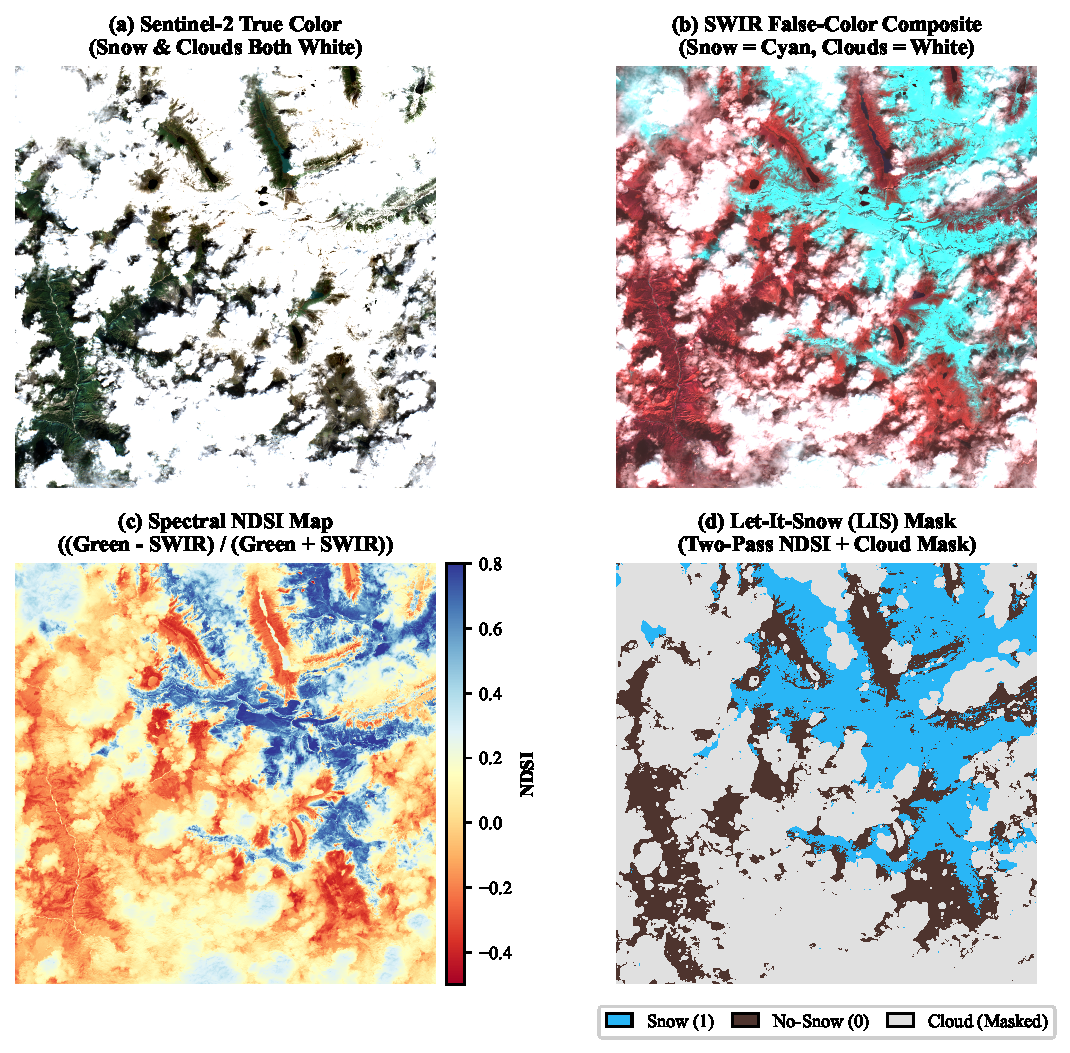
\includegraphics[width=0.78\textwidth]{figures/sentinel2_lis_pipeline_sample.pdf}
  \vspace{-6pt}
  \caption{Illustration of optical snow detection and cloud masking using Sentinel-2 L2A imagery over a $24\text{ km} \times 24\text{ km}$ Himalayan window. \textbf{(a)} True-color RGB (snow and clouds both appear bright white). \textbf{(b)} SWIR false-color composite ($\text{B11}/\text{B4}/\text{B3}$), separating snow (cyan) from clouds (white). \textbf{(c)} Normalized Difference Snow Index ($\text{NDSI}$). \textbf{(d)} Output Let-It-Snow (\texttt{LIS}) weak label mask.}
  \label{fig:s2_lis_demo}
\end{figure}

\paragraph{Thresholding based SAR snow cover segmentation.}
Because microwaves penetrate clouds, SAR has been widely studied for snow monitoring. Liquid water in wet snow increases dielectric absorption, strongly attenuating C-band backscatter relative to a snow-free reference image. \citet{nagler2000retrieval} leveraged this to device a thresholding based snow cover algorithm. Since this depends on water content, dry snow is nearly transparent to C-band, so backscatter is dominated by the underlying ground \citep{briand2026weakly}. Multi-frequency SAR studies indicate that combining longer radar wavelengths (such as S-band or L-band) with C-band provides complementary sensitivity to snowpack structure, surface roughness, and wetness.

\paragraph{Deep learning based SAR snow segmentation.}
Recent works have replaced fixed thresholds with Convolutional Neural Networks (CNNs). \citet{le2023deep} trained machine learning and CNN models on Sentinel-1 backscatter ratios using optical fusion, with \citet{gallet2024wet} and \citet{daudt2023snow} demonstrating that incorporating topographic channels (elevation and slope) significantly reduces mountain classification errors. \citet{briand2026weakly} pioneered weakly supervised training of a U-Net to jointly segment both wet and dry snow solely from dual-pol Sentinel-1 SAR amplitude images supervised by optical labels. Notably, \citet{briand2026weakly} proved that concatenating winter backscatter with Rayleigh MLE summer references, outperformed explicit wet/dry ratio channels because dividing by the reference image strips away implicit topographic context.

\begin{table}[h]
  \caption{Comparison of closely related SAR snow cover mapping studies.}
  \label{tab:lit_comparison}
  \centering
  \small
  \begin{tabular}{p{0.20\linewidth}p{0.18\linewidth}p{0.18\linewidth}p{0.14\linewidth}p{0.20\linewidth}}
    \toprule
    Study & SAR Input & Supervision Source & Snow States & Key Limitation \\
    \midrule
    \citet{nagler2016advancements} & C-band ($\sigma^0/\sigma^0_{\text{ref}}$) & Fixed threshold & Wet only & Blind to dry snow \\
    \citet{lievens2019snow} & C-band $\sigma^0_{\text{VH}}/\sigma^0_{\text{VV}}$ & MODIS prior mask & Dry depth & Requires optical mask \\
    \citet{briand2026weakly} & C-band (4-ch) & MODIS NDSI & Wet \& Dry & Coarse resolution \\
    \textbf{Phase~I} & \textbf{C-band (6-ch)} & \textbf{S2 LIS NDSI} & \textbf{Wet \& Dry} & - \\
    \textbf{Phase~II} & \textbf{C+S band} & \textbf{S2 LIS} NDSI & \textbf{Wet \& Dry} & - \\
    \bottomrule
  \end{tabular}
\end{table}

\paragraph{Research gap.}
As summarized in Table~\ref{tab:lit_comparison}, the closest prior work by \citet{briand2026weakly} trained a C-band SAR network using coarse 500\,m MODIS labels over small European Alpine basins ($230\text{--}411\text{ km}^2$, elevations $1000\text{--}4000\text{ m}$) and intentionally omitted explicit DEM features, experiencing a sharp performance drop ($\text{F1}_{\text{Snow}}$ falling from 92.1\% on MODIS to 74.4\% on 20\,m Sentinel-2 LIS labels under spatial transfer). No prior work has:
\begin{enumerate}
    \item Trained a weakly supervised SAR snow segmentation network directly on native 20\,m Sentinel-2 LIS two-pass optical labels in the Himalayan Region
    \item Investigated whether S-band SAR is physically complementary to C-band SAR. S-band has never been widely available to public until this year. NISAR mission is the first of its kind to provide S-band data for public access which is why no prior work exists on this particular topic.
\end{enumerate}

%===============================================================================
\section{Problem Formulation}
\label{sec:formulation}

\guide{About half a page. Define the task formally: inputs, outputs, notation,
assumptions, and the evaluation metric(s) with their definitions. Explain why
each metric suits the problem (e.g., why macro-F1 rather than accuracy for
imbalanced classes). If your project is not a prediction task (e.g., a system,
an analysis or a dataset), state the research questions or hypotheses and how
each will be tested.}

Let $\mathbf{S}_t \in \mathbb{R}^{H \times W \times 2}$ denote a dual-polarization SAR acquisition at winter date $t$ over a spatial grid of height $H$ and width $W$ at 10\,m resolution, containing linear backscatter amplitudes $(\sigma^0_{\text{VV},t}, \sigma^0_{\text{VH},t})$. From a set of $N_{\text{sum}}$ summer acquisitions $\{t_1, \dots, t_{N_{\text{sum}}}\}$, we estimate a snow-free reference map $\mathbf{S}_{\text{ref}} = (\sigma^0_{\text{VV,ref}}, \sigma^0_{\text{VH,ref}}) \in \mathbb{R}^{H \times W \times 2}$ assuming a Rayleigh amplitude distribution \citep{briand2026weakly}. Let $\mathbf{D} = (Z, S) \in \mathbb{R}^{H \times W \times 2}$ denote the static topographic channels (normalized elevation $Z$ and slope $S$) derived from a co-registered Digital Elevation Model (DEM). Combining these yields a $C$-channel input tensor $\mathbf{X}_t \in \mathbb{R}^{H \times W \times C}$ ($C \in \{2, 4, 6\}$ for C-band experiments done in Phase-I).

During training, each scene is paired with a weak optical label map $\tilde{\mathbf{Y}}_t \in \{0, 1, 255\}^{H \times W}$ derived from coincident Sentinel-2 imagery via the Let-It-Snow algorithm \citep{simon2018algorithm}, where $0$ denotes confirmed snow-free ground, $1$ denotes snow cover, and $255$ denotes unobservable pixels (cloud cover, radar shadow/nodata, or summer permasnow). The goal is to learn a segmentation network $f_\theta : \mathbb{R}^{H_p \times W_p \times C} \rightarrow [0, 1]^{H_p \times W_p \times 2}$ on $256 \times 256$ patches by minimizing the class-weighted masked cross-entropy loss over valid pixels $\Omega_t = \{r \in \{1, \dots, H_p W_p\} \mid \tilde{y}_{t,r} \neq 255\}$:
\begin{equation}
  \mathcal{L}_{\text{WCE}}(\theta) = -\frac{1}{|\Omega_t|} \sum_{r \in \Omega_t} \Big[ w_1 \, \tilde{y}_{t,r} \log \hat{p}_{t,r} + w_0 \, (1 - \tilde{y}_{t,r}) \log (1 - \hat{p}_{t,r}) \Big],
  \label{eq:wce}
\end{equation}
where $\hat{p}_{t,r} = \text{softmax}(f_\theta(\mathbf{X}_t))_{r,1}$ is the predicted snow probability at pixel $r$, and $(w_0, w_1) = (0.2, 0.8)$ counteracts the severe minority-class imbalance of snow ($\sim 7.1\%$) in full Himalayan swaths.

\paragraph{Evaluation metrics.}
Given binary predictions $\hat{y}_r = \mathbb{I}(\hat{p}_r \ge \tau)$ at a validation-tuned threshold $\tau \in (0, 1)$ and cumulative confusion counts $(\text{TP}, \text{FP}, \text{FN}, \text{TN})$ over valid test pixels, we evaluate:
\begin{align}
  \text{F1}_{\text{Snow}} &= \frac{2\,\text{TP}}{2\,\text{TP} + \text{FP} + \text{FN}}, \quad
  \text{IoU}_{\text{Snow}} = \frac{\text{TP}}{\text{TP} + \text{FP} + \text{FN}}, \quad
  \text{Macro F1} = \frac{\text{F1}_{\text{Snow}} + \text{F1}_{\text{NoSnow}}}{2}, \label{eq:metrics1} \\
  \text{Overall F1} &= f_{\text{Snow}}\,\text{F1}_{\text{Snow}} + (1 - f_{\text{Snow}})\,\text{F1}_{\text{NoSnow}}, \quad \text{where } f_{\text{Snow}} = \frac{\text{TP} + \text{FN}}{\text{TP} + \text{FP} + \text{FN} + \text{TN}}. \label{eq:eq22}
\end{align}
Because full Himalayan swaths contain 85\%--94\% snow-free pixels (mostly in low-elevation valleys $<3000\text{ m}$), global Accuracy and frequency-weighted Overall F1 (Eq.~\ref{eq:eq22}, defined in \citealp{briand2026weakly}) are heavily dominated by $\text{F1}_{\text{NoSnow}}$. Therefore, $\text{F1}_{\text{Snow}}$, $\text{IoU}_{\text{Snow}}$, Macro F1, and elevation-stratified metrics ($<3000\text{ m}$, $3000\text{--}4000\text{ m}$, $4000\text{--}5000\text{ m}$, $>5000\text{ m}$) are chosen as  primary indicators of true snow segmentation quality.

%===============================================================================
\section{Data}
\label{sec:data}

\guide{About half to one page. Describe every dataset you use: source (with
citation or URL), size, what one sample looks like, label definitions, class
balance, licence or permission to use it, and any ethical concerns (personal
data, consent). Describe preprocessing and how you split the data into
train/validation/test (and how you avoid leakage, e.g., splitting by subject or
by time). Include one or two informative exploratory figures or a summary table.
If you collected data yourself, describe the collection protocol;
\citet{gebru2021datasheets} is a good checklist.}

A multi-sensor SAR dataset comprising 18 co-registered pairs of Sentinel-1A C-band SAR (IW GRDH, dual-pol VV+VH) and Sentinel-2 L2A multispectral optical scenes obtained from the European Space Agency (ESA) Copernicus Data Space Ecosystem (\url{https://dataspace.copernicus.eu/}), paired with the Copernicus 30\,m Global DEM (\texttt{COP-DEM\_GLO-30}). All satellite products are open-access under the Copernicus free and open data license and does not contain personal/human imagery hence no privacy concerns.

% \begin{table}[h]
%   \caption{Summary of the curated Himalayan multi-sensor datasets (10\,m UTM Zone 46N, EPSG:32646).}
%   \label{tab:data}
%   \centering
%   \small
%   \begin{tabular}{lrrrrl}
%     \toprule
%     Dataset Subset & Scenes & Grid Size ($W \times H$) & $256\times256$ Patches & Snow \% (Valid) & Median Snow Elev. \\
%     \midrule
%     Primary Summer Ref (\texttt{patch1--6}) & 6 & $27{,}669 \times 21{,}231$ & --- (MLE Ref) & Permasnow masked & --- \\
%     Primary Winter Train (\texttt{patch7--11}) & 5 & $27{,}669 \times 21{,}231$ & $41{,}515$ (stride 128) & 7.10\% & $5{,}169\text{ m}$ \\
%     Primary Winter Val (\texttt{patch12}) & 1 & $27{,}669 \times 21{,}231$ & $10{,}368$ (stride 256) & 6.07\% & $5{,}180\text{ m}$ \\
%     Test Summer Ref (\texttt{patch\_test/1--5}) & 5 & $15{,}349 \times 14{,}462$ & --- (MLE Ref) & Permasnow masked & --- \\
%     Test Winter Eval (\texttt{patch\_test/winter}) & 1 & $15{,}349 \times 14{,}462$ & $13{,}566$ (stride 128) & 14.88\% & $4{,}298\text{ m}$ \\
%     \bottomrule
%   \end{tabular}
% \end{table}

\begin{table}[htbp]
    \centering
    \caption{Summary of the curated Himalayan multi-sensor datasets (10\,m UTM Zone 46N, EPSG:32646).}
    \label{tab:data}
    \small
    \setlength{\tabcolsep}{4pt}

    \resizebox{\textwidth}{!}{%
    \begin{tabular}{lrrrrl}
        \toprule
        Dataset Subset & Scenes & Grid Size ($W \times H$) & $256\times256$ Patches & Snow \% (Valid) & Median Snow Elev. \\
        \midrule
        Primary Summer Ref (\texttt{patch1--6}) & 6 & $27{,}669 \times 21{,}231$ & (MLE Ref) & Permasnow masked & --- \\
        Primary Winter Train (\texttt{patch7--11}) & 5 & $27{,}669 \times 21{,}231$ & $133{,}256$ (stride 128) & 7.10\% & $5{,}169\,\mathrm{m}$ \\
        Primary Winter Val (\texttt{patch12}) & 1 & $27{,}669 \times 21{,}231$ & $10{,}368$ (stride 256) & 6.07\% & $5{,}180\,\mathrm{m}$ \\
        Test Summer Ref (\texttt{patch\_test/1--5}) & 5 & $15{,}349 \times 14{,}462$ & (MLE Ref) & Permasnow masked & --- \\
        Test Winter Eval (\texttt{patch\_test/winter}) & 1 & $15{,}349 \times 14{,}462$ & $10{,}748$ (stride 128) & 14.88\% & $4{,}298\,\mathrm{m}$ \\
        \bottomrule
    \end{tabular}%
    }
\end{table}

\paragraph{Preprocessing and leakage-free data splitting.}
As detailed in Table~\ref{tab:data} and illustrated in Figures~\ref{fig:data_prep}--\ref{fig:cloud_snow_stats}, all scenes are projected onto a common grid. Sentinel-2 optical scenes are processed via the Let-It-Snow algorithm \citep{simon2018algorithm} to generate training labels ($0=\text{NoSnow}$, $1=\text{Snow}$, $2=\text{Cloud}\rightarrow 255$, $255=\text{NoData}$). Sentinel-1 GRDH scenes are processed in ESA SNAP through restituted orbit refinement, thermal noise removal, radiometric $\sigma^0$ calibration, and Range-Doppler terrain correction at 10\,m spacing, followed by exact affine grid alignment and $256 \times 256$ internal block tiling. To prevent temporal or spatial leakage:
\begin{enumerate}
  \item \textbf{Temporal split (Primary Basin, $58{,}740\text{ km}^2$):} Summer scenes \texttt{patch1--6} compute the snow-free reference image; five winter scenes (\texttt{patch7--11}) form the training set; and one completely held-out winter date (\texttt{patch12}) forms the validation set (Figures~\ref{fig:winter_series} and~\ref{fig:cloud_snow_stats}).
  \item \textbf{Spatial transfer split (\texttt{patch\_test}, $22{,}200\text{ km}^2$):} An independent Himalayan massif with its own 5-scene summer MLE reference (\texttt{patch1--5}) and unseen winter evaluation scene. Exploratory elevation analysis (Table~\ref{tab:data} and Figure~\ref{fig:shift_plot}) reveals a major physical domain shift: the median snow elevation in \texttt{patch\_test} is $4{,}298\text{ m}$ (10th--90th percentile: $3{,}768\text{--}4{,}909\text{ m}$), which is $871\text{ m}$ lower than in the training basin ($5{,}169\text{ m}$, 10th--90th percentile: $4{,}382\text{--}5{,}946\text{ m}$).
\end{enumerate}

\begin{figure}[!htbp]
  \centering
  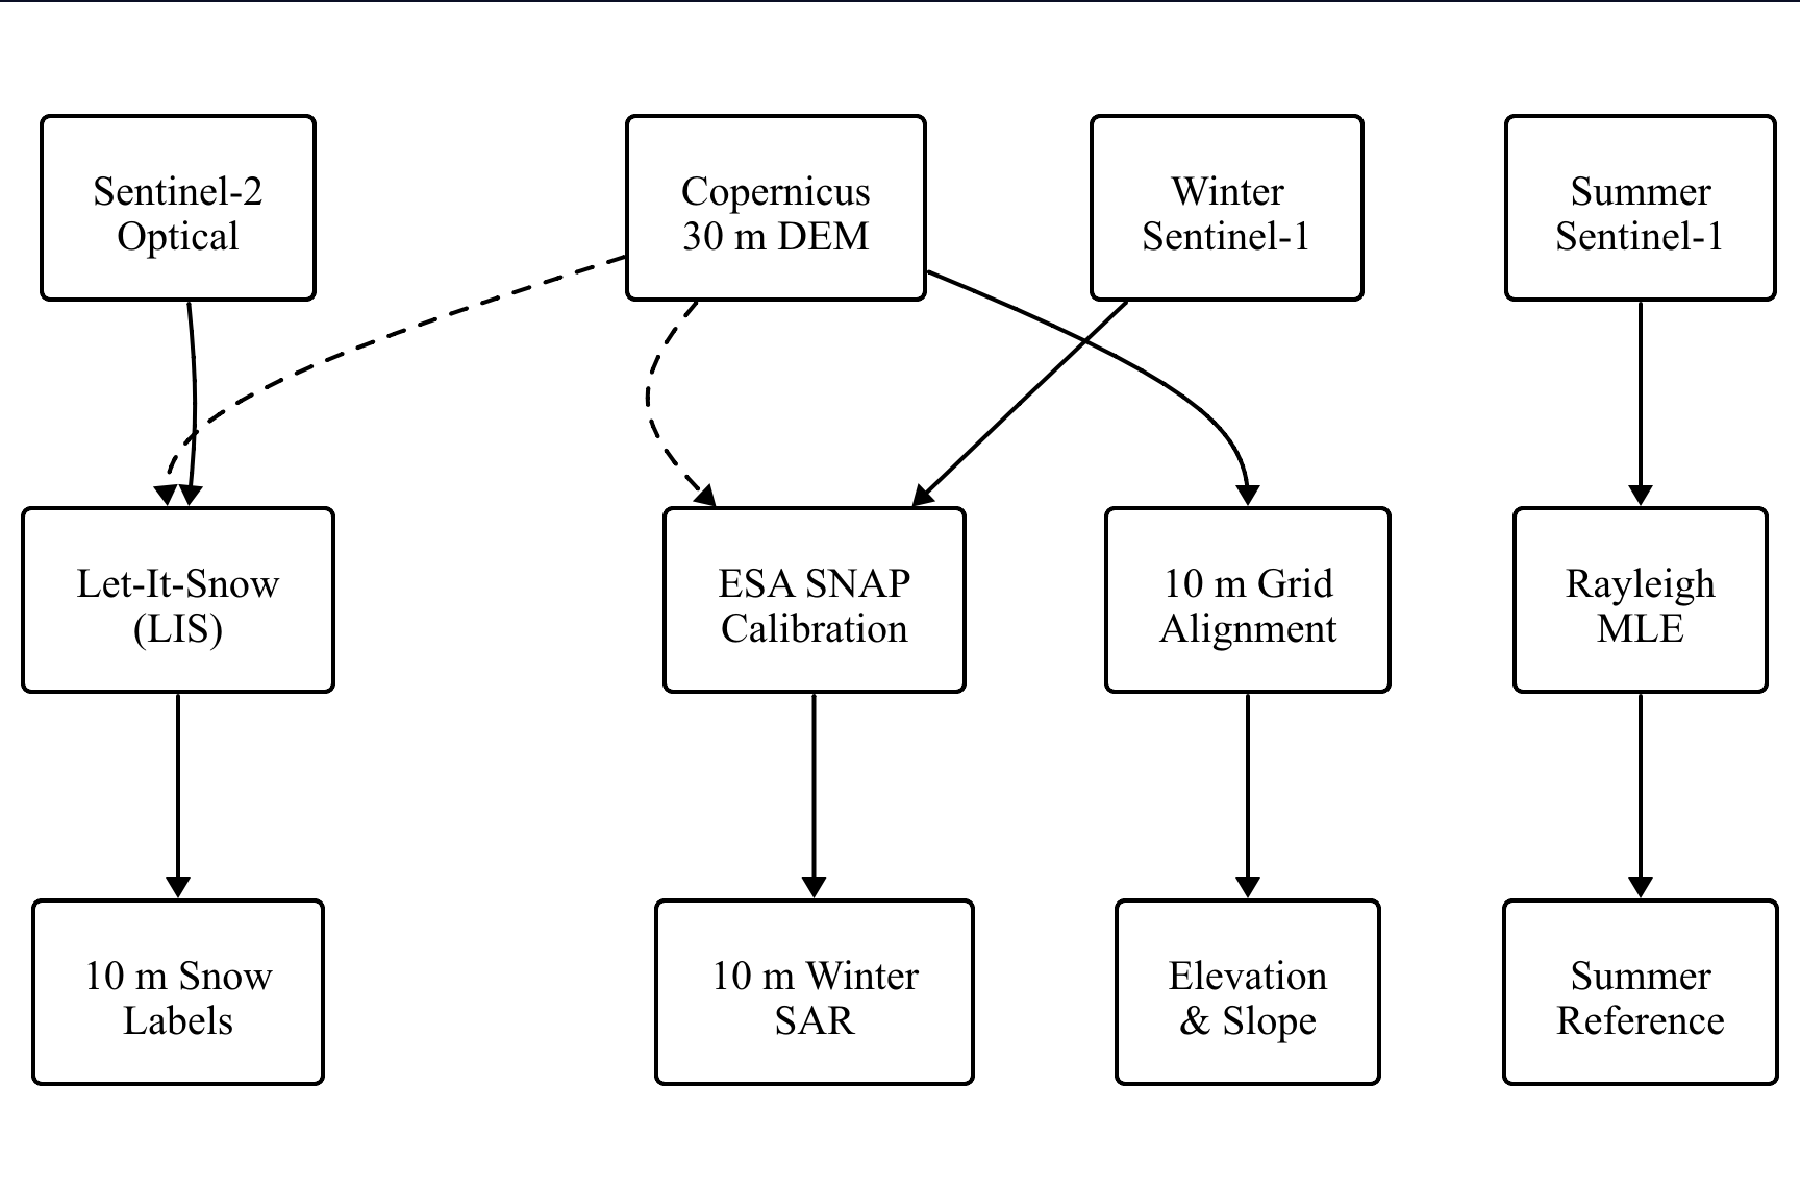
\includegraphics[width=0.68\textwidth]{figures/data_preprocessing_diagram.pdf}
  \vspace{-6pt}
  \caption{Multi-sensor preprocessing and 10\,m grid alignment workflow.}
  \label{fig:data_prep}
\end{figure}

\begin{figure}[!htbp]
  \centering
  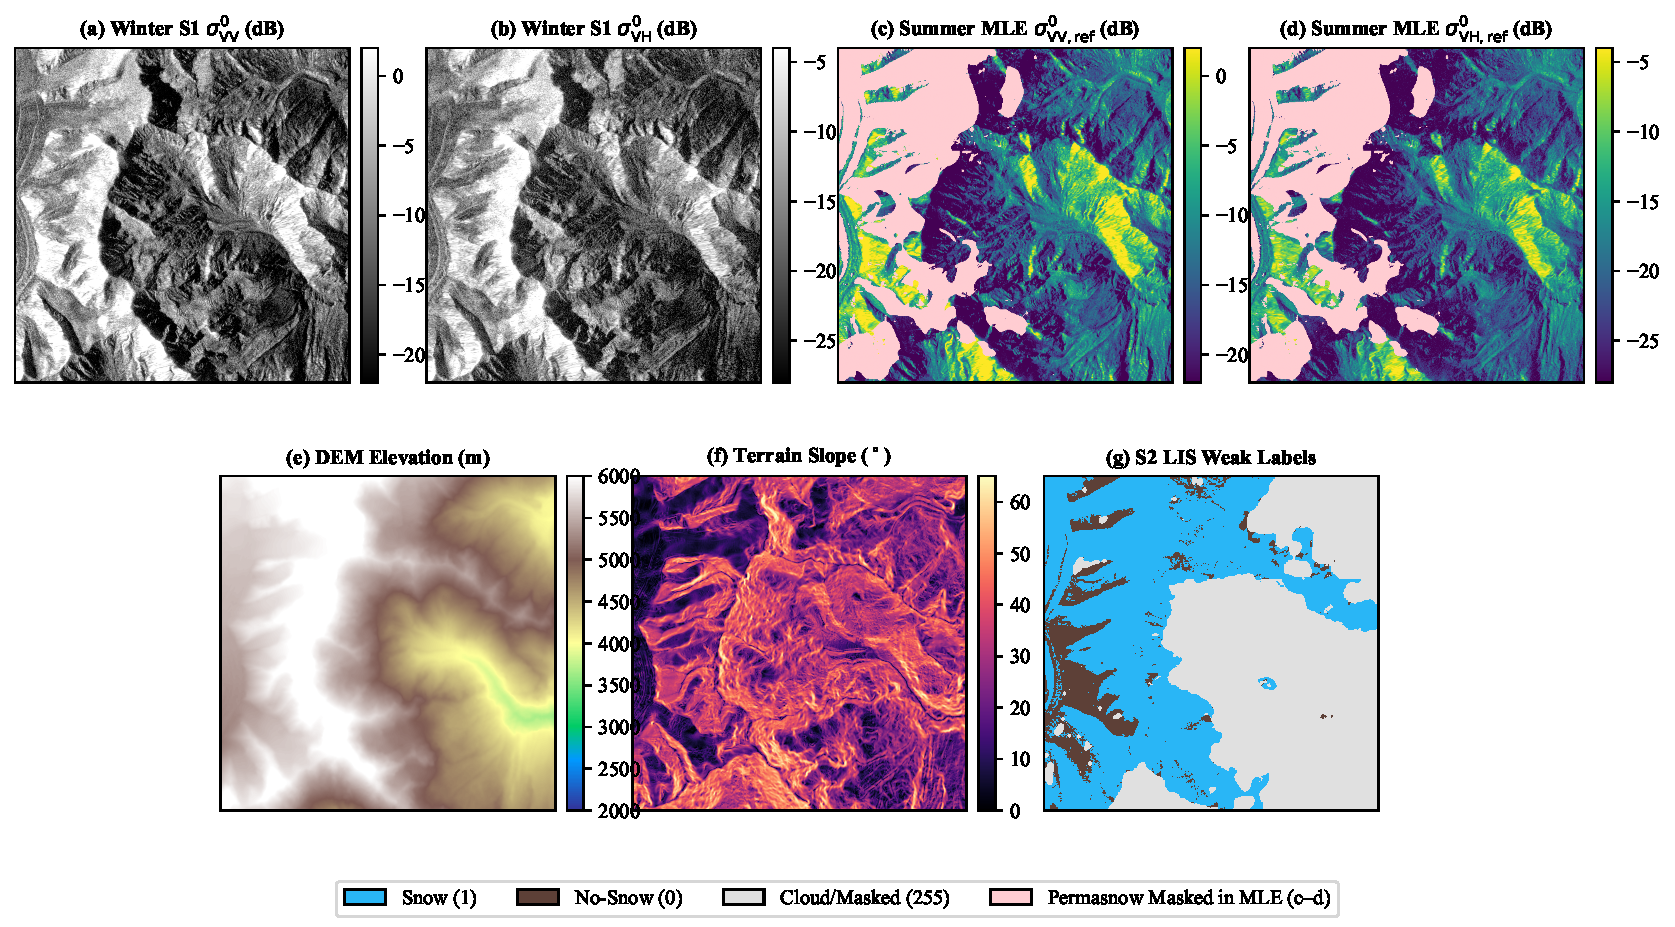
\includegraphics[width=0.92\textwidth]{figures/sample_satellite_data.pdf}
  \vspace{-6pt}
  \caption{Sample co-registered multi-sensor inputs and optical weak labels over a $10.24\text{ km} \times 10.24\text{ km}$ window in \texttt{patch12} (10\,m grid). \textbf{(a--b)} Winter Sentinel-1 C-band backscatter ($\sigma^0_{\text{VV}}, \sigma^0_{\text{VH}}$). \textbf{(c--d)} Permasnow-masked Rayleigh MLE summer reference ($\sigma^0_{\text{VV,ref}}, \sigma^0_{\text{VH,ref}}$). \textbf{(e)} Multi-temporal SAR composite. \textbf{(f--g)} Copernicus DEM elevation and slope. \textbf{(h)} Sentinel-2 \texttt{LIS} weak labels.}
  \label{fig:sample_data}
\end{figure}

% \begin{figure}[!htbp]
%   \centering
%   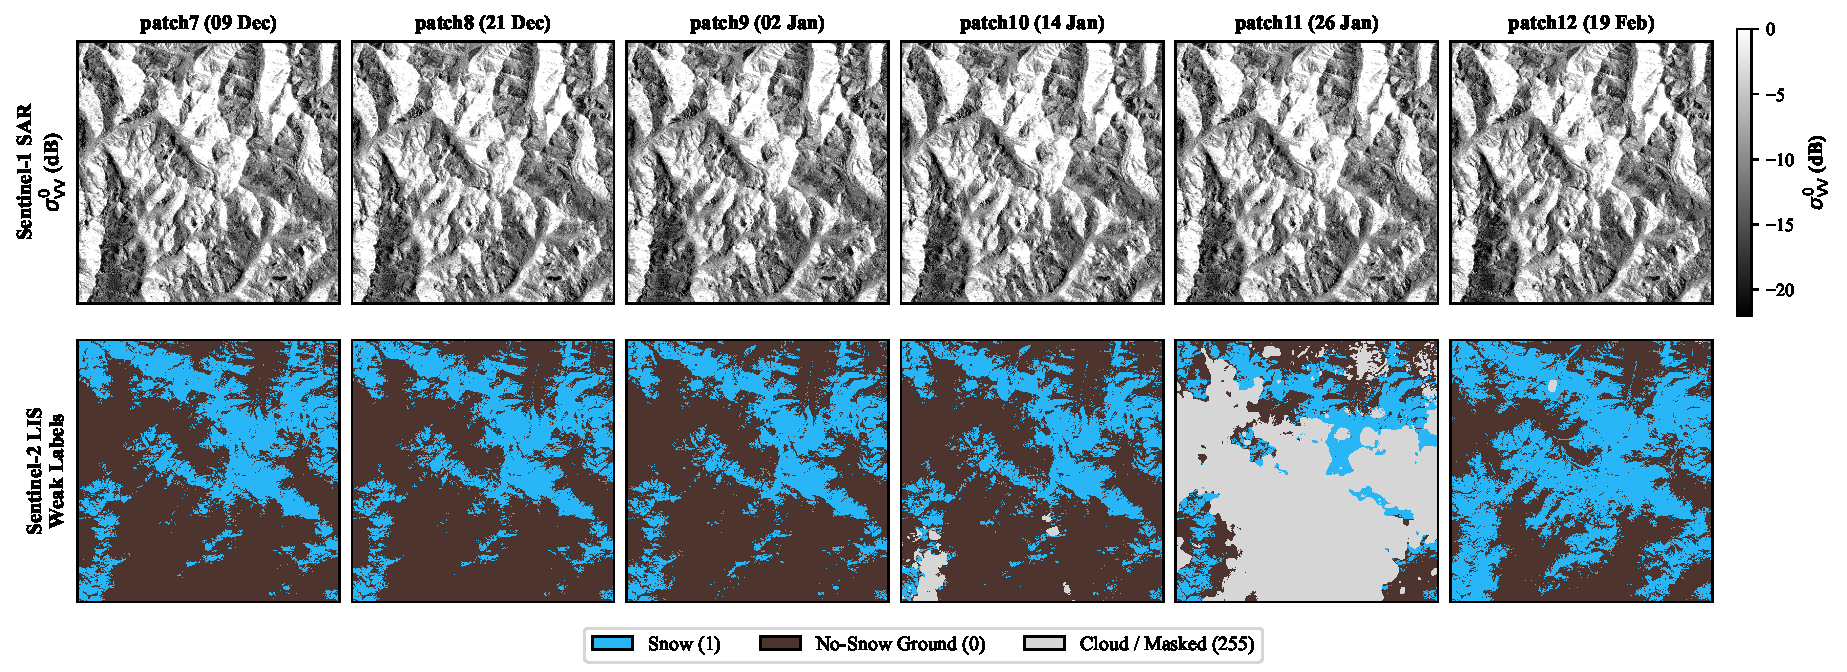
\includegraphics[width=0.98\textwidth]{figures/multitemporal_winter_series.pdf}
%   \vspace{-6pt}
%   \caption{Multi-temporal winter series across \texttt{patch7}--\texttt{patch12} (09 Dec to 19 Feb) over a $20.48\text{ km} \times 20.48\text{ km}$ high-alpine subregion. \textbf{(Top)} Cloud-penetrating Sentinel-1 SAR $\sigma^0_{\text{VV}}$ (dB). \textbf{(Bottom)} Coincident Sentinel-2 \texttt{LIS} weak labels, illustrating heavy cloud obscuration on \texttt{patch11} (26 Jan) while SAR remains unobstructed.}
%   \label{fig:winter_series}
% \end{figure}

\begin{figure}[!htbp]
  \centering
  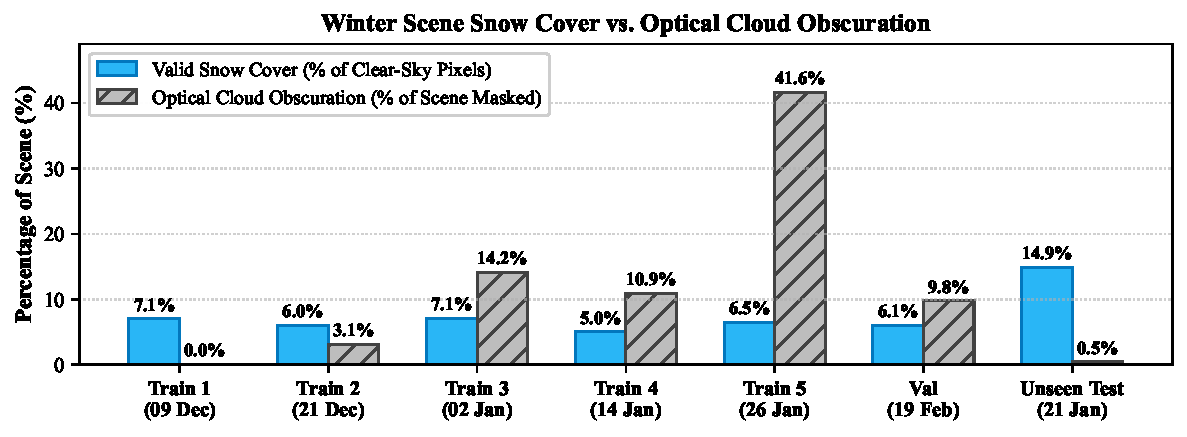
\includegraphics[width=0.68\textwidth]{figures/scene_cloud_snow_plot.pdf}
  \vspace{-6pt}
  \caption{Scene-wise valid snow cover percentage versus optical cloud obscuration across the winter training (\texttt{patch7--11}), validation (\texttt{patch12}), and unseen test (\texttt{patch\_test}) acquisitions.}
  \label{fig:cloud_snow_stats}
\end{figure}

%===============================================================================
\section{Methodology}
\label{sec:method}

\guide{About one page. Describe (i) the baseline method(s) you compare against and
why they are appropriate, and (ii) your proposed approach, with enough detail
that another student could implement it. A block diagram of the pipeline
(Figure~\ref{fig:pipeline}) is strongly recommended. If the proposed method is
not finalised yet, describe the candidate approaches and how you will choose
between them. Clearly separate what already exists (cite it) from what is your
own contribution.}

% \begin{figure}[h]
%   \centering
%   \fbox{\begin{minipage}{0.95\linewidth}
%     \centering\footnotesize\vspace{4pt}
%     \textbf{Stage 1: Multi-Sensor Preprocessing \& Reference Estimation}\\
%     Sentinel-2 L2A + DEM $\xrightarrow{\text{Docker Let-It-Snow \citep{simon2018algorithm}}}$ 10\,m Labels $\tilde{\mathbf{Y}}_t \in \{0, 1, 255\}$ (Clouds Masked as 255)\\
%     Summer Sentinel-1 (\texttt{patch1--6}) $\xrightarrow{\text{Rayleigh MLE + Permasnow Mask}}$ $\sigma^0_{\text{VV,ref}}, \sigma^0_{\text{VH,ref}}$ (\texttt{S1A\_MLE\_Reference.tif})\\
%     Winter Sentinel-1 + DEM $\xrightarrow{\text{SNAP } \sigma^0 \text{ + Terrain Corr. + Alignment}}$ $\sigma^0_{\text{VV},t}, \sigma^0_{\text{VH},t}, Z_{\text{norm}}, S_{\text{norm}}$\\[6pt]
%     \textbf{Stage 2: Weakly Supervised U-Net Ablation \& Gaussian-Weighted Inference}\\
%     Input Stack $\mathbf{X}_t$ (\textbf{Step 1:} 2-ch $[\text{VV}, \text{VH}]$ $\mid$ \textbf{Step 2:} 4-ch $+[\text{VV}_{\text{ref}}, \text{VH}_{\text{ref}}]$ $\mid$ \textbf{Step 3:} 6-ch $+[Z_{\text{norm}}, S_{\text{norm}}]$)\\
%     $\longrightarrow$ 3-Stage U-Net $\xrightarrow{\text{Masked WCE Loss } [0.2, 0.8]}$ Val Threshold Selection (\texttt{patch12}) $\longrightarrow$ Gaussian Overlap Test Inference
%     \vspace{4pt}
%   \end{minipage}}
%   \caption{Overview of the Phase~I weakly supervised SAR snow cover segmentation pipeline. Optical \texttt{LIS} labels supervise training only; at test inference, only SAR, summer MLE reference, and DEM channels are required.}
%   \label{fig:pipeline}
% \end{figure}

\begin{figure}[!htbp]
  \centering
  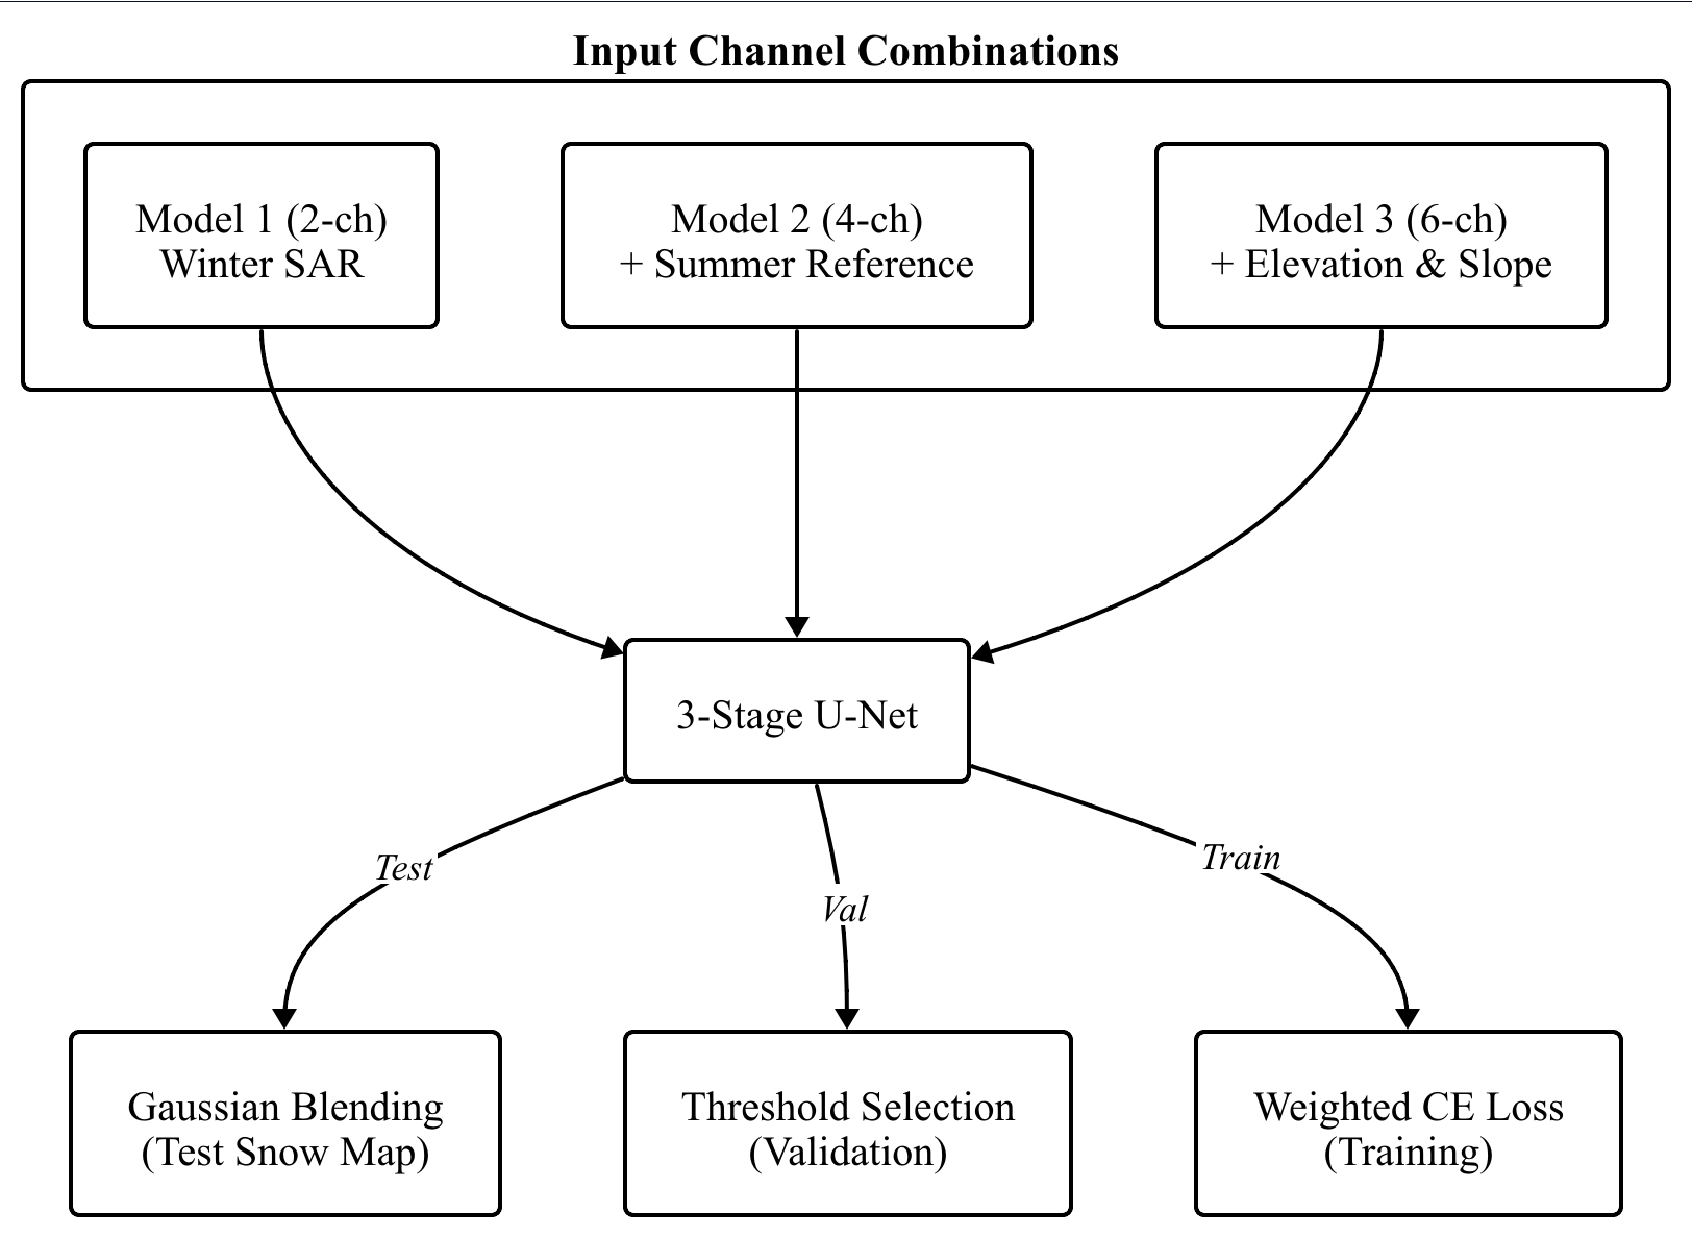
\includegraphics[width=0.66\textwidth]{figures/pipeline_diagram.pdf}
  \vspace{-4pt}
  \caption{Overview of the Phase~I weakly supervised SAR snow cover segmentation pipeline. Optical LIS labels supervise training only; at test inference, only SAR, summer MLE reference, and DEM channels are required.}
  \label{fig:pipeline}
\end{figure}

\paragraph{Baseline and benchmark configurations.}
This approach was benchmarked against the weakly supervised framework of \citet{briand2026weakly}. The baseline (Model~1: Channel Set~A) trains a 3-stage U-Net \citep{ronneberger2015unet} on 2-channel raw winter C-band backscatter $(\sigma^0_{\text{VV}}, \sigma^0_{\text{VH}})$ normlized and converted to decibels.

\paragraph{Rayleigh MLE and topographic fusion (Model~2 and~3).}
As illustrated in Figure~\ref{fig:pipeline}, two progressive physical enhancements over the raw SAR baseline were introduced:
\begin{enumerate}
  \item \textbf{Permasnow-Masked Rayleigh MLE Reference (Step~2: Channel Set~B, 4 channels):} Following \citet{briand2026weakly}, the snow-free reference images were calculated via the Rayleigh MLE across $N(h,w)$ summer observations for each polarization $p \in \{\text{VH}, \text{VV}\}$:
  \begin{equation}
    \sigma^0_{p,\text{ref}}(h, w) = \sqrt{\frac{1}{2\,N(h,w)} \sum_{t=1}^{N(h,w)} \big(\sigma^0_{p,t}(h,w)\big)^2}.
    \label{eq:mle}
  \end{equation}
  Unlike the French Alps in \citet{briand2026weakly} ($<4000\text{ m}$), Himalayan peaks above $5200\text{ m}$ retain permanent snow and glaciers in July--August. Hence, this implementation masks any pixel where \texttt{LIS} labels indicate snow, accumulating strictly confirmed clear-sky snow-free observations and cloud-penetrating summer SAR only where permanent snow never occurs. This yields the 4-channel Set~B stack: $[\text{VV}, \text{VH}, \text{VV}_{\text{ref}}, \text{VH}_{\text{ref}}]$ (see physical backscatter contrast distributions in Figure~\ref{fig:sar_dist}).
  \item \textbf{Topographic Channel Fusion (Model~3: Set~B + DEM, 6 channels):} Addressing the discussion in \citet[Section~6.1]{briand2026weakly}, two terrain channels were computed from the 10\,m aligned and normalized DEM altitude and slope forming a 6-channel input tensor.
  \item \textbf{Controlled U-Net Architecture and Gaussian Inference:} All models use an identical from-scratch 3-stage U-Net ($C \rightarrow 64 \rightarrow 128 \rightarrow 256$ channels, $3\times3$ convolutions, BatchNorm, ReLU) so that performance differences isolate input channel properties rather than pretraining biases. At test inference, $256\times256$ predictions at stride 128 are blended with a 2D Gaussian kernel).
\end{enumerate}

\begin{figure}[!htbp]
  \centering
  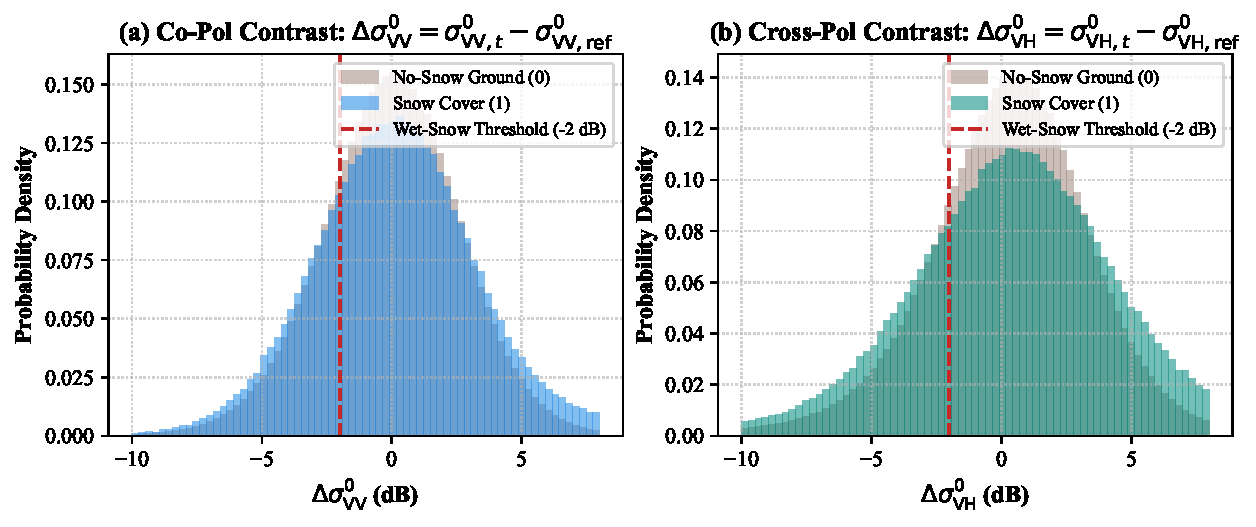
\includegraphics[width=0.78\textwidth]{figures/sar_backscatter_distribution_plot.pdf}
  \vspace{-6pt}
  \caption{Empirical probability density of winter-minus-summer C-band SAR backscatter contrast ($\Delta\sigma^0_{\text{VV}}$ and $\Delta\sigma^0_{\text{VH}}$ in dB on \texttt{patch12}) for Snow versus No-Snow ground relative to the classical $-2\text{ dB}$ wet-snow threshold \citep{nagler2000retrieval}.}
  \label{fig:sar_dist}
\end{figure}

%===============================================================================
\section{Experiments and Preliminary Results}
\label{sec:results}

\guide{About 1.5--2 pages. Report only
what you have actually run. Preliminary or negative results are acceptable and
should be reported honestly. If you have no results yet, report your
experimental setup in full and any pilot experiments, and explain what blocked
progress.}

\subsection{Experimental setup}
All models were implemented in PyTorch~2.6 using \texttt{rasterio} for windowed GeoTIFF streaming and trained on Google Colab (NVIDIA T4 GPU, 16\,GB VRAM) using mixed precision (\texttt{float16}), batch size 32, the Adam optimizer ($\text{lr} = 10^{-4}$), masked weighted cross-entropy loss ($w_0=0.2, w_1=0.8, \text{ignore\_index}=255$), and fixed random seeds (\texttt{seed} $= 42$) for 15 epochs ($\sim 25\text{ min}$ per model). Following \citet{briand2026weakly}, no geometric or intensity augmentations were applied. After each epoch, the classification threshold $\tau \in \{0.10, 0.15, \dots, 0.90\}$ maximizing $\text{F1}_{\text{Snow}}$ on the validation set (\texttt{patch12}) was stored in checkpoints and kept strictly fixed during evaluation on \texttt{patch\_test}.

\subsection{Results}
Table~\ref{tab:results} presents the quantitative results across all three C-band configurations on both the same-basin temporal validation set and the unseen spatial transfer test set, alongside the Channel Set~B benchmarks from \citet[Tables~4, 6, and~7]{briand2026weakly}. Table~\ref{tab:elevation_results} reports the elevation-stratified breakdown which is key result needed for Phase-II, and Figure~\ref{fig:model_outputs} compares the predicted snow maps qualitatively across both regions. \textbf{Stratified results have not be provided by prior weakly supervised SAR segmentation studies like \citep{briand2026weakly}} because overall performance of the model matters more but in this particular case, this stratified breakdown will help us prove that S-band SAR is indeed a complementary addition to C-band SAR, thus making this table an essential result for this research.

% \begin{table}[h]
%   \caption{Ablation results on same-basin temporal validation (\texttt{patch12}) and unseen-basin spatial transfer (\texttt{patch\_test}) at fixed validation thresholds, compared with \citet{briand2026weakly}. Best Phase~I results in bold.}
%   \label{tab:results}
%   \centering
%   \small
%   \begin{tabular}{llcccccc}
%     \toprule
%     Scenario \& Method & Channels & $\text{F1}_{\text{Snow}}$ ($\uparrow$) & $\text{IoU}_{\text{Snow}}$ ($\uparrow$) & Macro F1 ($\uparrow$) & Overall F1 ($\uparrow$) & Prec.\ ($\uparrow$) & Rec.\ ($\uparrow$) \\
%     \midrule
%     \multicolumn{8}{l}{\emph{A. Same-Basin Temporal Generalization (\texttt{patch12} vs.\ Briand Guil 2018)}} \\
%     \citet{briand2026weakly} (S2 \texttt{LIS} Eval) & Set~B (4-ch) & 84.70\% & 0.7346 & 80.30\% & 81.50\% & --- & --- \\
%     Step~1: Raw C-Band (Baseline) & Set~A (2-ch) & 56.84\% & 0.3970 & 77.02\% & 94.80\% & 54.73\% & 59.12\% \\
%     Step~2: C-Band + Summer MLE & Set~B (4-ch) & 67.10\% & 0.5049 & 82.58\% & 96.25\% & \textbf{72.21\%} & 62.66\% \\
%     Step~3: C-Band + MLE + DEM & Set~B+DEM (6-ch) & \textbf{69.27\%} & \textbf{0.5299} & \textbf{83.68\%} & \textbf{96.48\%} & 66.39\% & \textbf{72.42\%} \\
%     \midrule
%     \multicolumn{8}{l}{\emph{B. Unseen-Basin Spatial Transfer (\texttt{patch\_test} vs.\ Briand Gyronde 2018 on S2 \texttt{LIS})}} \\
%     \citet{briand2026weakly} (S2 \texttt{LIS} Eval) & Set~B (4-ch) & 74.40\% & 0.5924 & 71.05\% & 71.30\% & --- & --- \\
%     Step~1: Raw C-Band (Baseline) & Set~A (2-ch) & 43.34\% & 0.2767 & 68.18\% & 87.08\% & 49.63\% & \textbf{38.47\%} \\
%     Step~2: C-Band + Summer MLE & Set~B (4-ch) & 46.46\% & 0.3026 & 70.79\% & 89.27\% & \textbf{82.97\%} & 32.26\% \\
%     Step~3: C-Band + MLE + DEM & Set~B+DEM (6-ch) & \textbf{50.42\%} & \textbf{0.3371} & \textbf{72.82\%} & \textbf{89.83\%} & 79.35\% & 36.95\% \\
%     \bottomrule
%   \end{tabular}
% \end{table}

% \begin{table}[h]
%   \caption{Elevation-stratified snow segmentation performance on the unseen test massif (\texttt{patch\_test}).}
%   \label{tab:elevation_results}
%   \centering
%   \small
%   \begin{tabular}{llccc}
%     \toprule
%     Elevation Zone (\texttt{patch\_test}) & Metric & Step~1: Set~A (2-ch) & Step~2: Set~B (4-ch) & Step~3: Set~B + DEM (6-ch) \\
%     \midrule
%     $<3000\text{ m}$ (Snow-Free Valleys) & Accuracy ($\text{F1}_{\text{NoSnow}}$) & 96.42\% & 99.93\% & \textbf{100.00\%} \\
%     $3000\text{--}4000\text{ m}$ (Lower Transition) & $\text{F1}_{\text{Snow}}$ / $\text{IoU}_{\text{Snow}}$ & 25.35\% / 0.1451 & 24.73\% / 0.1411 & \textbf{25.87\%} / \textbf{0.1486} \\
%     $4000\text{--}5000\text{ m}$ (Mid-Alpine Zone) & $\text{F1}_{\text{Snow}}$ / $\text{IoU}_{\text{Snow}}$ & 50.97\% / 0.3420 & 51.32\% / 0.3452 & \textbf{55.35\%} / \textbf{0.3827} \\
%     $>5000\text{ m}$ (High-Alpine Core) & $\text{F1}_{\text{Snow}}$ / $\text{IoU}_{\text{Snow}}$ & \textbf{73.08\%} / \textbf{0.5758} & 66.79\% / 0.5014 & 70.29\% / 0.5420 \\
%     \bottomrule
%   \end{tabular}
% \end{table}

% \begin{table}[h]
%   \caption{Model metrics on same-basin temporal validation and unseen-basin spatial transfer at fixed validation thresholds, compared with \citet{briand2026weakly}. Best Phase~I results in bold.}
%   \label{tab:results}
%   \centering
%   \resizebox{\textwidth}{!}{%
%   \begin{tabular}{llcccccc}
%     \toprule
%     Scenario \& Method & Channels & $\text{F1}_{\text{Snow}}$ ($\uparrow$) & $\text{IoU}_{\text{Snow}}$ ($\uparrow$) & Macro F1 ($\uparrow$) & Overall F1 ($\uparrow$) & Prec.\ ($\uparrow$) & Rec.\ ($\uparrow$) \\
%     \midrule
%     \multicolumn{8}{l}{\emph{A. Same-Basin Temporal Generalization}} \\
%     \citet{briand2026weakly} & Set~B (4-ch) & \textbf{84.70\%} & \textbf{0.7346} & 80.30\% & 81.50\% & --- & --- \\
%     Model~1: Raw C-Band (Baseline) & Set~A (2-ch) & 56.84\% & 0.3970 & 77.02\% & 94.80\% & 54.73\% & 59.12\% \\
%     Model~2: C-Band + Summer MLE & Set~B (4-ch) & 67.10\% & 0.5049 & 82.58\% & 96.25\% & \textbf{72.21\%} & 62.66\% \\
%     Model~3: C-Band + MLE + DEM & Set~B+DEM (6-ch) & 69.27\% & 0.5299 & \textbf{83.68\%} & \textbf{96.48\%} & 66.39\% & \textbf{72.42\%} \\
%     \midrule
%     \multicolumn{8}{l}{\emph{B. Unseen-Basin Spatial Transfer}} \\
%     \citet{briand2026weakly} (S2 & Set~B (4-ch) & \textbf{74.40\%} & \textbf{0.5924} & 71.05\% & 71.30\% & --- & --- \\
%     Model~1: Raw C-Band (Baseline) & Set~A (2-ch) & 43.34\% & 0.2767 & 68.18\% & 87.08\% & 49.63\% & \textbf{38.47\%} \\
%     Model~2: C-Band + Summer MLE & Set~B (4-ch) & 46.46\% & 0.3026 & 70.79\% & 89.27\% & \textbf{82.97\%} & 32.26\% \\
%     Model~3: C-Band + MLE + DEM & Set~B+DEM (6-ch) & 50.42\% & 0.3371 & \textbf{72.82\%} & \textbf{89.83\%} & 79.35\% & 36.95\% \\
%     \bottomrule
%   \end{tabular}%
%   }
% \end{table}

\begin{table}[!htbp]
  \caption{Model metrics on same-basin temporal validation and unseen-basin spatial transfer at fixed validation thresholds, compared with \citet{briand2026weakly}. Best Phase~I results in bold.}
  \label{tab:results}
  \centering
  \resizebox{\textwidth}{!}{%
  \begin{tabular}{llcccc}
    \toprule
    Scenario \& Method & Channels & $\text{F1}_{\text{Snow}}$ ($\uparrow$) & $\text{IoU}_{\text{Snow}}$ ($\uparrow$) & Macro F1 ($\uparrow$) & Overall F1 ($\uparrow$) \\
    \midrule
    \multicolumn{6}{l}{\emph{A. Same-Basin Temporal Generalization}} \\
    \citet{briand2026weakly} & Set~B (4-ch) & \textbf{84.70\%} & \textbf{0.7346} & 80.30\% & 81.50\% \\
    Model~1: Raw C-Band (Baseline) & Set~A (2-ch) & 56.84\% & 0.3970 & 77.02\% & 94.80\% \\
    Model~2: C-Band + Summer MLE & Set~B (4-ch) & 67.10\% & 0.5049 & 82.58\% & 96.25\% \\
    Model~3: C-Band + MLE + DEM & Set~B+DEM (6-ch) & 69.27\% & 0.5299 & \textbf{83.68\%} & \textbf{96.48\%} \\
    \midrule
    \multicolumn{6}{l}{\emph{B. Unseen-Basin Spatial Transfer}} \\
    \citet{briand2026weakly} & Set~B (4-ch) & \textbf{74.40\%} & \textbf{0.5924} & 71.05\% & 71.30\% \\
    Model~1: Raw C-Band (Baseline) & Set~A (2-ch) & 43.34\% & 0.2767 & 68.18\% & 87.08\% \\
    Model~2: C-Band + Summer MLE & Set~B (4-ch) & 46.46\% & 0.3026 & 70.79\% & 89.27\% \\
    Model~3: C-Band + MLE + DEM & Set~B+DEM (6-ch) & 50.42\% & 0.3371 & \textbf{72.82\%} & \textbf{89.83\%} \\
    \bottomrule
  \end{tabular}%
  }
\end{table}

\begin{table}[!htbp]
  \caption{Elevation-stratified snow segmentation performance on the unseen test massif (\texttt{patch\_test}).}
  \label{tab:elevation_results}
  \centering
  \resizebox{\textwidth}{!}{%
  \begin{tabular}{llccc}
    \toprule
    Elevation Zone (\texttt{patch\_test}) & Metric & Model~1 (2-ch) & Model~2 (4-ch) & Model~3 (6-ch) \\
    \midrule
    $<3000\text{ m}$ (Snow-Free Valleys) & Accuracy ($\text{F1}_{\text{NoSnow}}$) & 96.42\% & 99.93\% & \textbf{100.00\%} \\
    $3000\text{--}4000\text{ m}$ (Lower Transition) & $\text{F1}_{\text{Snow}}$ / $\text{IoU}_{\text{Snow}}$ & 25.35\% / 0.1451 & 24.73\% / 0.1411 & \textbf{25.87\%} / \textbf{0.1486} \\
    $4000\text{--}5000\text{ m}$ (Mid-Alpine Zone) & $\text{F1}_{\text{Snow}}$ / $\text{IoU}_{\text{Snow}}$ & 50.97\% / 0.3420 & 51.32\% / 0.3452 & \textbf{55.35\%} / \textbf{0.3827} \\
    $>5000\text{ m}$ (High-Alpine Core) & $\text{F1}_{\text{Snow}}$ / $\text{IoU}_{\text{Snow}}$ & \textbf{73.08\%} / \textbf{0.5758} & 66.79\% / 0.5014 & 70.29\% / 0.5420 \\
    \bottomrule
  \end{tabular}%
  }
\end{table}

\begin{figure}[!htbp]
  \centering
  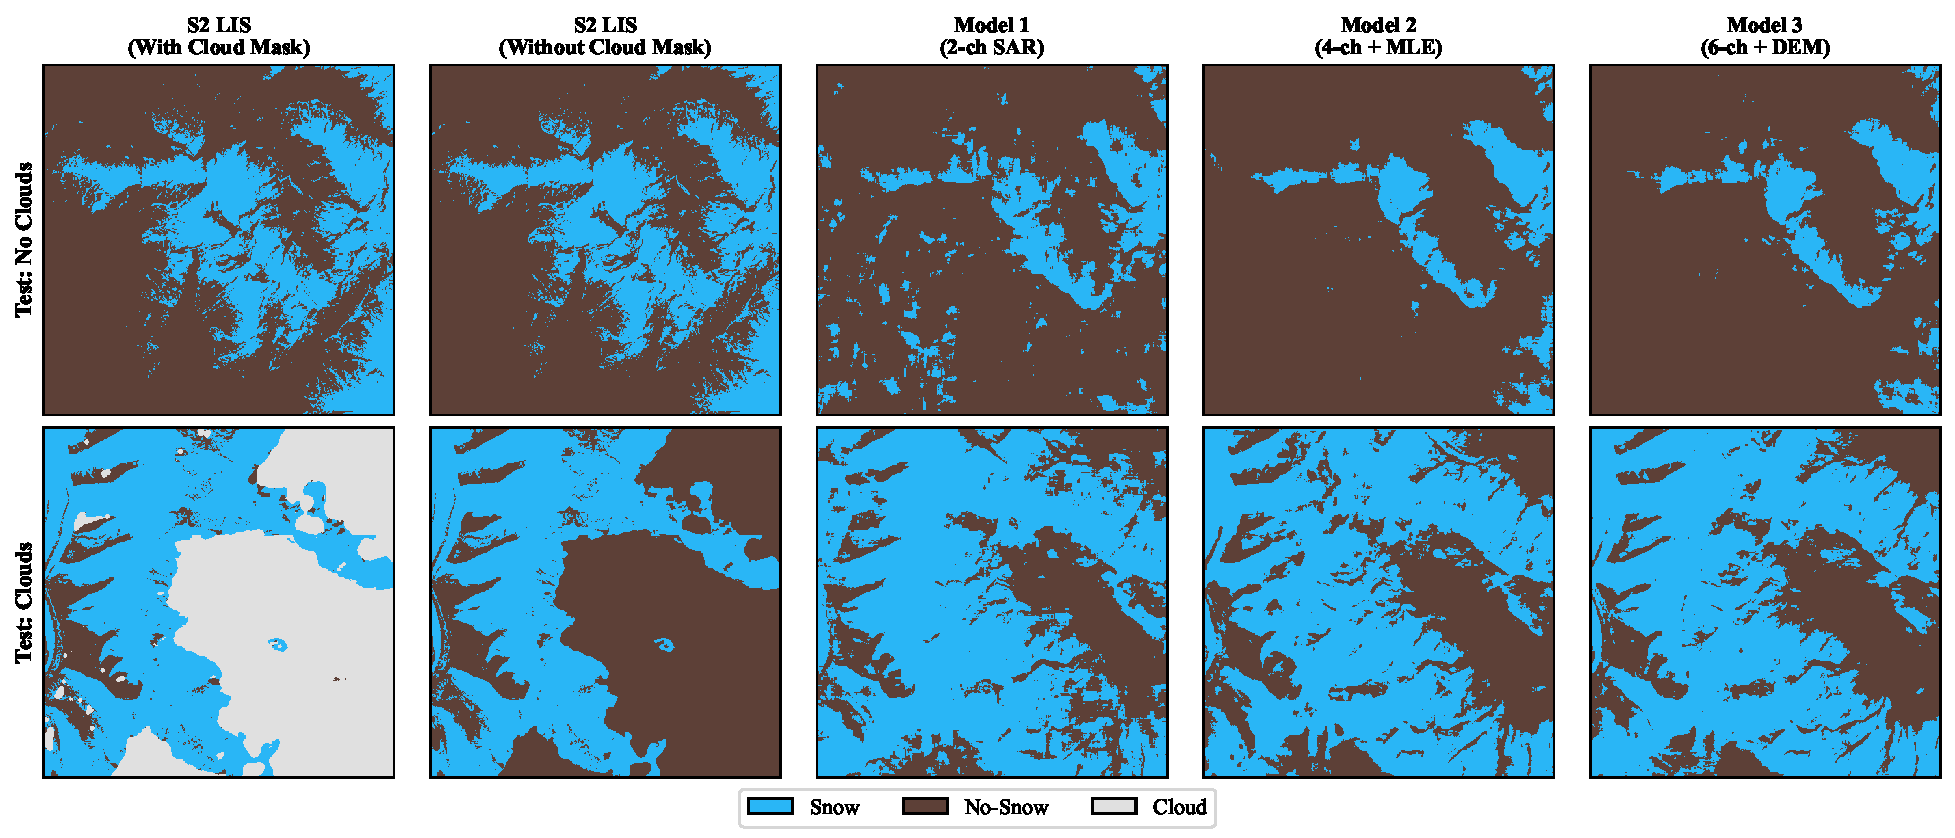
\includegraphics[width=0.95\textwidth]{figures/model_outputs_comparison.pdf}
  \vspace{-4pt}
  \caption{Qualitative comparison of snow segmentation outputs across the three C-band U-Net configurations on \textbf{(Top)} the validation scene (\texttt{patch12}) and \textbf{(Bottom)} the unseen test massif (\texttt{patch\_test}). Columns show: (1) Copernicus DEM elevation, (2) Sentinel-2 \texttt{LIS} ground truth, (3--5) binary predictions for Models~1, 2, and~3, and (6) pixel-wise error agreement map for Model~3 (TP, TN, FP, FN).}
  \label{fig:model_outputs}
\end{figure}

\subsection{Analysis}
\paragraph{Impact of Rayleigh MLE reference and DEM features.} Adding the snow-free summer MLE reference (Model 2) yields a $+10.26\%$ jump in validation $\text{F1}_{\text{Snow}}$ (56.84\% $\rightarrow$ 67.10\%) and boosts test Precision from 49.63\% to 82.97\% ($+33.34\%$, Figure~\ref{fig:pr_comp}). By comparing winter backscatter against the snow-free terrain baseline, the network suppresses false alarms caused by rough snow-free boulders and radar shadow. Adding normalized elevation and slope (Model~3) further improves validation ($\text{F1}_{\text{Snow}} = 69.27\%$) and unseen test $\text{F1}_{\text{Snow}}$ from 46.46\% to 50.42\% ($\text{Macro F1} = 72.82\%$). Across elevation bands (Table~\ref{tab:elevation_results} and Figure~\ref{fig:elev_plot}), Model~3 achieves 100.00\% accuracy below $3000\text{ m}$ (eliminating all low-elevation radar layover false positives), improves mid-alpine ($4000\text{--}5000\text{ m}$) $\text{F1}_{\text{Snow}}$ by $+4.03\%$ (51.32\% $\rightarrow$ 55.35\%), and reaches $70.29\%$ $\text{F1}_{\text{Snow}}$ above $5000\text{ m}$.

\begin{figure}[!htbp]
  \centering
  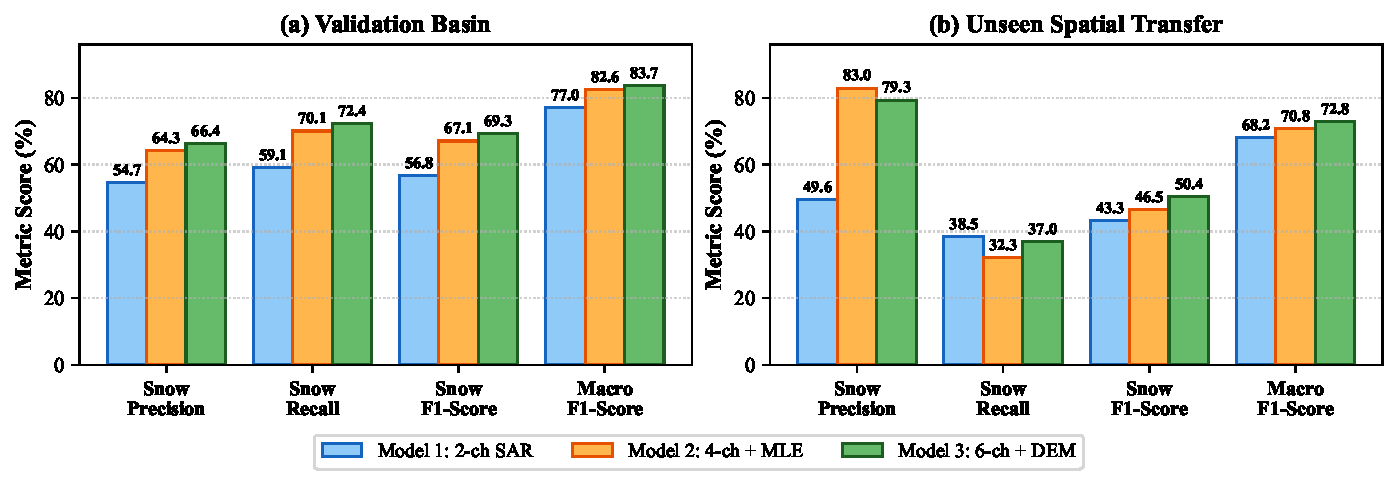
\includegraphics[width=0.80\textwidth]{figures/precision_recall_comparison_plot.pdf}
  \vspace{-6pt}
  \caption{Comparison of Snow Precision, Snow Recall, $\text{F1}_{\text{Snow}}$, and Macro F1 across Models~1, 2, and~3 on \textbf{(a)} validation (\texttt{patch12}) and \textbf{(b)} unseen spatial transfer (\texttt{patch\_test}).}
  \label{fig:pr_comp}
\end{figure}

\begin{figure}[!htbp]
  \centering
  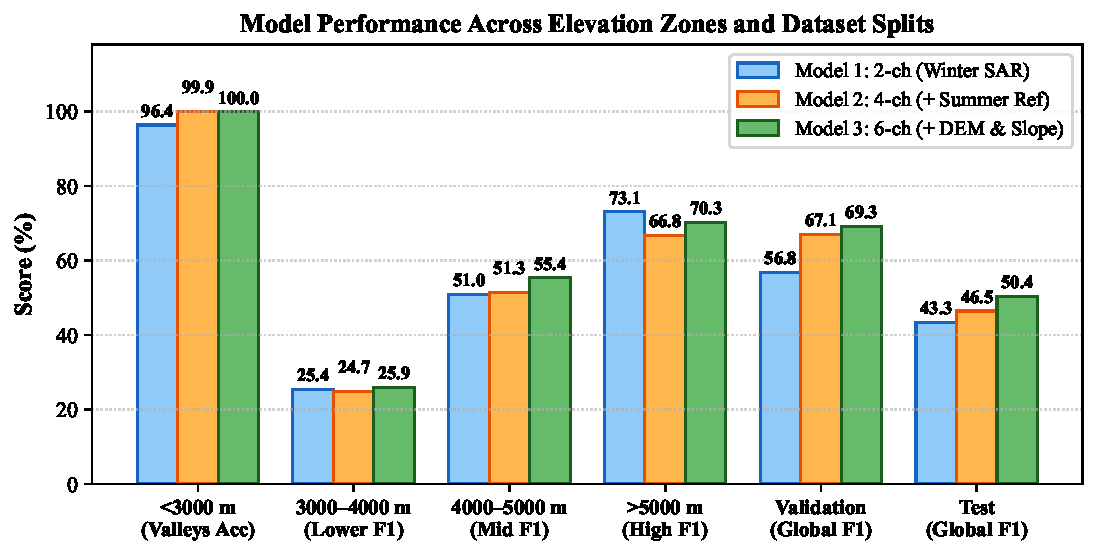
\includegraphics[width=0.62\textwidth]{figures/elevation_performance_plot.pdf}
  \vspace{-6pt}
  \caption{Progression of elevation-stratified and global snow segmentation metrics across Models~1, 2, and~3.}
  \label{fig:elev_plot}
\end{figure}

\begin{figure}[!htbp]
  \centering
  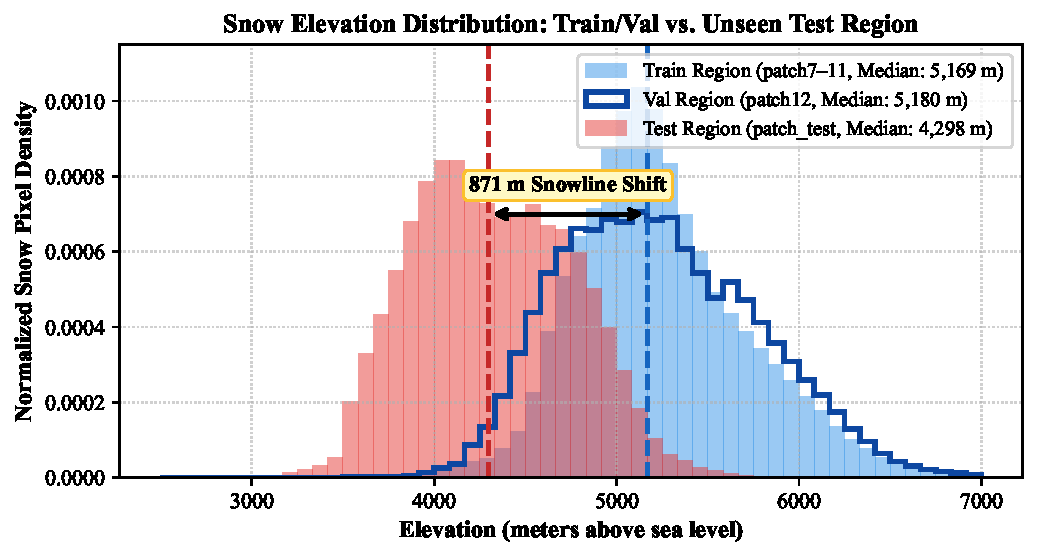
\includegraphics[width=0.62\textwidth]{figures/domain_shift_plot.pdf}
  \vspace{-6pt}
  \caption{Empirical snow elevation distribution across training (\texttt{patch7--11}), validation (\texttt{patch12}), and unseen test (\texttt{patch\_test}) sets, showing the $871\text{ m}$ snowline shift.}
  \label{fig:shift_plot}
\end{figure}

\paragraph{Comparison with \citet{briand2026weakly} and error analysis.}
Although the global frequency-weighted Overall F1 (89.83\% on \texttt{patch\_test}) appears numerically higher than \citet{briand2026weakly}'s spatial-transfer Overall F1 on Sentinel-2 \texttt{LIS} labels (71.30\%, Table~\ref{tab:results}), this is an artifact of class imbalance in Equation~\ref{eq:eq22}: our full Himalayan swath is 85.12\% No-Snow, whereas \citet{briand2026weakly}'s cropped Alpine basin was 61.6\% Snow. On the true positive-class metric ($\text{F1}_{\text{Snow}}$), our baseline U-Net (50.42\% global, 55.35\% at $4000\text{--}5000\text{ m}$, 70.29\% at $>5000\text{ m}$) scores below \citet{briand2026weakly} (74.40\% spatial transfer) for the following reasons: (i) Finegrained resolution, \citet{briand2026weakly} trained and evaluated their model on $20m \times 20m$ resolution ($500m \times 500m$ MODIS labels were upscaled) on cropped Alpine basin (1,000m - 4,000m elevation) where as the current model was trained on $10m \times 10m$ ($20m \times 20m$ Sentinel 2 LIS labels were upscaled) resolution across uncropped 58,740 $km^2$. Drop in metrics is expected as resolution increases because the model needs to learn more information and is prone to make more mistakes. (ii) \emph{Snowline shift} (Figures~\ref{fig:shift_plot} and~\ref{fig:thresh_sens}): snow in \texttt{patch\_test} occurs at a median elevation of $4298\text{ m}$ vs.\ $5169\text{ m}$ in training, causing conservative probabilities in the $3500\text{--}4500\text{ m}$ zone; (iii) \emph{time-series density:} These models were trained on 5 single-orbit dates vs.\ 88 multi-orbit dates in \citet{briand2026weakly}; and (iv) \emph{C-band dry/wet transition ambiguity and sparse-vegetation impact} at $3000\text{--}4500\text{ m}$, is a motivating factor for S-band fusion in Phase~II.

% \begin{figure}[!htbp]
%   \centering
%   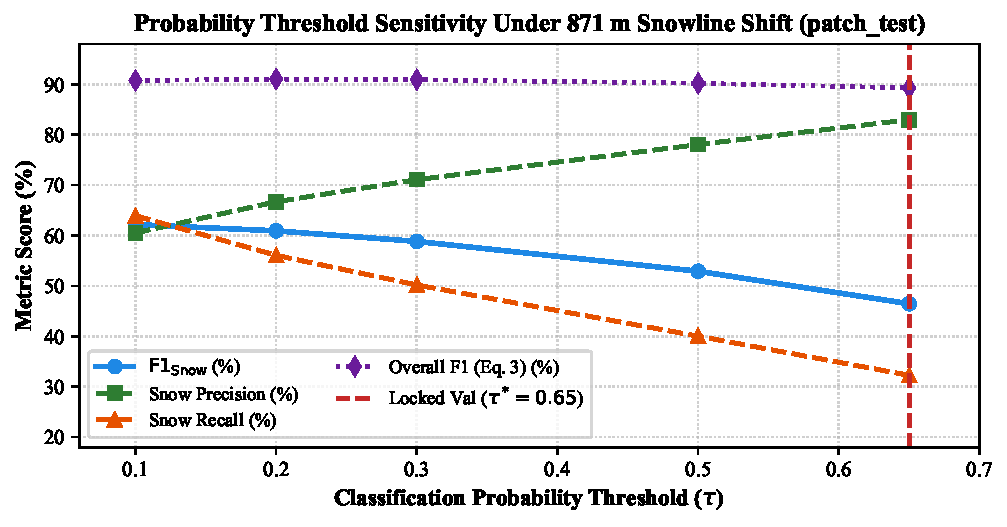
\includegraphics[width=0.64\textwidth]{figures/threshold_sensitivity_plot.pdf}
%   \vspace{-6pt}
%   \caption{Diagnostic probability threshold sensitivity on \texttt{patch\_test} (4-ch Set~B), showing how the $871\text{ m}$ snowline shift affects Recall and $\text{F1}_{\text{Snow}}$ at the locked validation threshold ($\tau^\ast = 0.65$).}
%   \label{fig:thresh_sens}
% \end{figure}

%===============================================================================
\section{Discussion and Limitations}
\label{sec:discussion}

\guide{About half a page. What do the Phase~I results tell you about the
original plan? Has the problem or approach changed since the start of the
semester, and why? State the limitations of the current work (data, method,
evaluation) honestly.}

Phase~I study confirms the core hypothesis: weakly supervised training on 10\,m Sentinel-2 \texttt{LIS} labels successfully transfers snow segmentation capability to C-band SAR, and every physical input addition (raw SAR $\rightarrow$ +MLE $\rightarrow$ +MLE+DEM) monotonically improves both in-domain validation ($\text{F1}_{\text{Snow}}$: $56.84\% \rightarrow 67.10\% \rightarrow 69.27\%$) and out-of-domain spatial transfer ($43.34\% \rightarrow 46.46\% \rightarrow 50.42\%$).

\paragraph{Limitations.}
First, Phase~I training set uses only 5 single-orbit winter scenes unlike \citet{briand2026weakly} who trained the model on 88 dates. This is done because S-band data availability started this year (2026), training the model with 88 C-band dates and 5 S-band dates will cause the model to learn C-band data more and not pay enough attention to S-band data. Second, C-band SAR alone struggles to detect shallow dry snow due to short wavelength in mid-elevation transition zones, directly motivating the Phase~II integration of S-band SAR.

%===============================================================================
\section{Plan for Semester IV}
\label{sec:plan}

\guide{About half to one page. Give a concrete, dated plan linked to the
objectives in Table~\ref{tab:objectives}. Each milestone should have a clear
deliverable. Also list the main risks (e.g., data access, compute, a method not
working) and your fallback for each. The Phase~II evaluation will check
progress against this plan.}

In Semester~IV (Phase~II), priority would be realizing the objectives O3, O4, and O5 mentioned in the milestone schedule in Table~\ref{tab:plan} and illustrated in Figure~\ref{fig:phase2_fusion}.

\paragraph{Risks and mitigation.}
\begin{itemize}
  \item \textbf{Risk 1 (Temporal/spatial alignment between S-band and C-band SAR acquisitions):} S-band and C-band acquisitions may differ in revisit dates or viewing incidence angles. \emph{Mitigation:} Co-register both sensors onto the exact 10\,m Copernicus DEM UTM grid using Range-Doppler terrain correction and normalize each sensor by its own orbit-specific Rayleigh MLE snow-free summer reference ($\sigma^0_{\text{S,ref}}, \sigma^0_{\text{C,ref}}$).
  \item \textbf{Risk 2 (Regional snowline elevation overfitting across mountain ranges):} Absolute elevation $Z/6000$ can suppress recall when testing on a basin with a lower snowline. \emph{Mitigation:} Replace or augment absolute elevation with relative elevation and local incidence angle maps during C+S fusion.
\end{itemize}

\begin{figure}[!htbp]
  \centering
  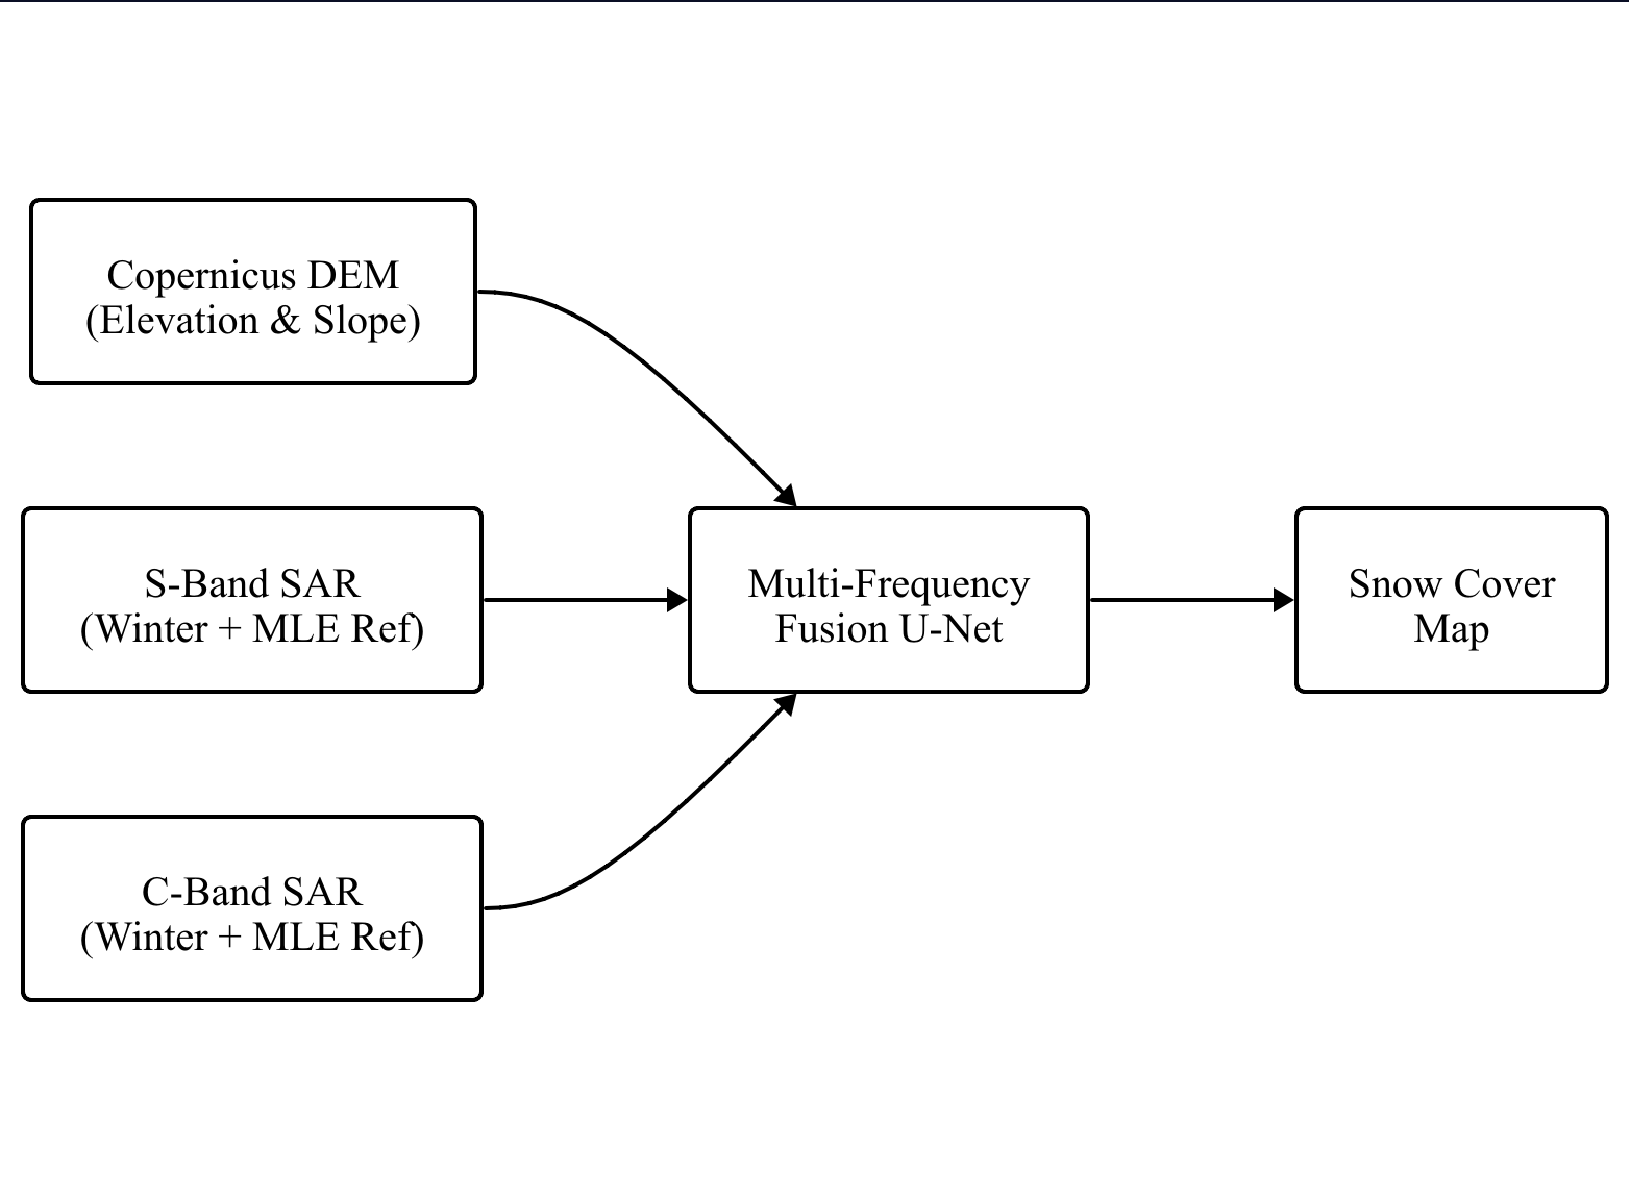
\includegraphics[width=0.58\textwidth]{figures/phase2_fusion_diagram.pdf}
  \vspace{-4pt}
  \caption{Planned Phase~II multi-frequency C-band + S-band fusion workflow.}
  \label{fig:phase2_fusion}
\end{figure}

\begin{table}[!htbp]
  \caption{Work plan for Semester IV (January--May 2027).}
  \label{tab:plan}
  \centering
  \small
  \begin{tabular}{p{0.16\linewidth}p{0.06\linewidth}p{0.44\linewidth}p{0.26\linewidth}}
    \toprule
    Period & Obj. & Task & Deliverable \\
    \midrule
    Jan 2027      & O3 & Preprocess S-band SAR scenes, co-register to 10\,m UTM grid, build S-band summer MLE reference, and train standalone S-band U-Net baseline. & Standalone S-band vs.\ C-band evaluation table \\
    Feb--Mar 2027 & O4 & Implement multi-frequency C-band + S-band fusion (input-level concatenation and dual-branch feature fusion + DEM) and evaluate across elevation zones. & Trained C+S fusion model \& complementarity ablation \\
    Apr 2027      & O5 & Package the code in an application with Graphical User Interface such that it could be used for demonstration purposes & Deliver demo \\
    May 2027      & --- & Thesis writing and submission. & Final M.Tech.\ Thesis \& Defense Presentation \\
    \bottomrule
  \end{tabular}
\end{table}

%===============================================================================
\section{Conclusion}
\label{sec:conclusion}

\guide{One paragraph. Restate the problem, what Phase~I has established, and the
single most important goal for Semester IV. No new information here.}

This project addresses all-weather, high-resolution (10\,m) seasonal snow cover segmentation in the Himalayas by transferring weak optical supervision from Sentinel-2 Let-It-Snow masks to cloud-penetrating dual-polarization SAR imagery. In Phase~I, an end-to-end preprocessing and training pipeline was built across 18 Himalayan scenes ($>58{,}740\text{ km}^2$) and demonstrated through a controlled U-Net study that augmenting raw C-band Sentinel-1 backscatter with permasnow-masked Rayleigh MLE summer references and DEM features (elevation and slope) improves snow F1-score. The primary goal for Semester~IV is to integrate S-band SAR with the C-band pipeline to prove multi-frequency C+S band complementarity in the mid-alpine transition zone and establish whether this improves snow cover estimation quality or not.

%===============================================================================
% Unnumbered sections below do not count towards the 10-page limit.
\newpage

% \begin{ack}
% The author gratefully acknowledges the supervision and guidance of the thesis supervisors at the Indian Institute of Technology Guwahati, the European Space Agency (ESA) Copernicus programme for open-access Sentinel-1, Sentinel-2, and Copernicus DEM data, and the Centre d'\'Etudes Spatiales de la Biosph\`ere (CESBIO) for the open-source Let-It-Snow (\texttt{LIS}) software.
% \end{ack}

\section*{Declaration on the use of AI tools}
\guide{Mandatory. State which AI tools (e.g., chatbots, code assistants,
writing tools) you used and for what (e.g., coding help, language editing,
literature search). If none, write ``No AI tools were used.'' You remain
responsible for every statement, citation and number in this report; check
every AI-suggested reference exists.}
\begin{itemize}
    \item No AI assistance was used for writing this report.
    \item AI coding assistant (Gemini/Antigravity) was used for coding and debugging.
\end{itemize}

\section*{Code and data availability}
All preprocessing, training, and evaluation scripts are maintained in the project GitHub. All raw Sentinel-1, Sentinel-2, and Copernicus DEM datasets are publicly available through the ESA Copernicus Data Space Ecosystem (\url{https://dataspace.copernicus.eu/}).

\bibliographystyle{plainnat}
\bibliography{references}

%===============================================================================
\appendix

% \section{Additional results}
\guide{Optional. Extra figures, tables, derivations or hyperparameter details.
The main text must stand on its own; evaluators are not required to read the
appendix.}

% Table~\ref{tab:appendix_sweep} reports the diagnostic probability threshold sweep on the unseen test massif (\texttt{patch\_test}) for the 4-channel (\texttt{with\_mle.pth}) model, illustrating the effect of the $871\text{ m}$ snowline domain shift on optimal probability thresholding between validation (\texttt{patch12}, where $\tau^\ast = 0.65$) and out-of-domain test terrain (where $\text{F1}_{\text{Snow}}$ peaks at $62.17\%$ for $\tau = 0.10$ and $52.91\%$ for $\tau = 0.50$).

% \begin{table}[h]
%   \caption{Diagnostic probability threshold sensitivity on \texttt{patch\_test} for Step~2 (\texttt{with\_mle.pth}, 4-ch Set~B). Note: test reporting in Table~\ref{tab:results} strictly uses the locked validation threshold $\tau^\ast = 0.65$.}
%   \label{tab:appendix_sweep}
%   \centering
%   \small
%   \begin{tabular}{cccccc}
%     \toprule
%     Threshold $\tau$ & Overall F1 (Eq.~\ref{eq:eq22}) & $\text{F1}_{\text{Snow}}$ & Snow Precision & Snow Recall & $\text{IoU}_{\text{Snow}}$ \\
%     \midrule
%     0.10 & 90.76\% & 62.17\% & 60.52\% & 63.92\% & 0.4511 \\
%     0.20 & 91.03\% & 60.93\% & 66.70\% & 56.07\% & 0.4381 \\
%     0.30 & 90.91\% & 58.83\% & 71.08\% & 50.18\% & 0.4167 \\
%     0.50 (Default) & 90.19\% & 52.91\% & 78.05\% & 40.02\% & 0.3597 \\
%     0.65 (Val Locked $\tau^\ast$) & 89.27\% & 46.46\% & 82.97\% & 32.26\% & 0.3026 \\
%     \bottomrule
%   \end{tabular}
% \end{table}

\section{Report checklist}
\guide{Mandatory. Before submitting, answer each item with \textbf{[Yes]},
\textbf{[No]} or \textbf{[NA]}, and add a one-line justification for any [No].}

{\footnotesize
\begin{enumerate}
  \item The problem statement and objectives are stated clearly in
        Section~\ref{sec:intro}, and each objective has a status in
        Table~\ref{tab:objectives}. \textbf{[Yes]}
  \item The literature review is organised by theme and ends with a stated
        research gap. \textbf{[Yes]}
  \item Every dataset's source, size, splits and licence/permission are
        reported. \textbf{[Yes]}
  \item At least one baseline is reported, or the absence of a baseline is
        justified. \textbf{[Yes]}
  \item Hyperparameters and model selection used only training/validation data;
        the test set was not used for tuning. \textbf{[Yes]}
  \item Results state the metric, the number of runs and their variation where
        applicable. \textbf{[Yes]}
  \item The Semester IV plan has dated milestones and deliverables.
        \textbf{[Yes]}
  \item Every figure and table is referred to in the text and has an
        informative caption. \textbf{[Yes]}
  \item Every reference is cited in the text, and every cited work has been
        checked to exist. \textbf{[Yes]}
  \item All guidance boxes have been removed (\texttt{\textbackslash showguidefalse}
        is set), and no template placeholder text remains. \textbf{[Yes]}
  \item The Conclusion section ends within the first 10 pages. \textbf{[Yes]}
  \item The AI-use declaration is filled in and the report complies with the
        institute's plagiarism policy. \textbf{[Yes]}
  \item I have received approval of this report from both my supervisors.
        \textbf{[Pending]}
\end{enumerate}
}

\end{document}
